\documentclass[letterpaper,12pt]{article}

\usepackage{tabularx} % extra features for tabular environment
\usepackage{amsmath}  % improve math presentation
\usepackage{graphicx} % takes care of graphic including machinery
\usepackage[margin=1in,letterpaper]{geometry} % decreases margins
\usepackage{cite} % takes care of citations
\usepackage[final]{hyperref} % adds hyper links inside the generated pdf file
\usepackage{ctex}
\usepackage{titlesec}
\usepackage{CJKutf8, CJK}
\usepackage{makecell}                 % 三线表-竖线
\usepackage{booktabs}                 % 三线表-短细横线
\usepackage{natbib}
\usepackage{graphicx}				  % 表格单元格逆时针
\usepackage{multirow}				  % 合并单元格
\usepackage{array}
\usepackage{amssymb}				  % 勾
\usepackage{longtable}                % 导入 longtable 宏包,表格自动换行
\usepackage{caption}
\usepackage{subcaption}               % 设置子图
\usepackage{color}					  % 文本颜色包
\usepackage{xcolor}
\usepackage{bbm}					  % 输入指示函数

\hypersetup{
	colorlinks=true,       % false: boxed links; true: colored links
	linkcolor=blue,        % color of internal links
	citecolor=blue,        % color of links to bibliography
	filecolor=magenta,     % color of file links
	urlcolor=blue         
}
%++++++++++++++++++++++++++++++++++++++++
\titleformat{\section}{\Large\bfseries\songti}{\thesection}{1em}{}
\titleformat{\subsection}{\large\bfseries\songti}{\thesubsection}{1em}{}
\titleformat{\subsubsection}{\normalsize\bfseries\songti}{\thesubsubsection}{1em}{}

\begin{document}
	
	
	\title{\songti \zihao{4}4月17日-4月23日工作汇报}
	\author{\textrm{Ku Jui}}
	\date{\textrm{April 2023}}
	\maketitle
	
	\renewcommand{\figurename}{Figure} % 可以重新定义abstract,因为ctex会覆盖thebibliography
% 	\begin{abstract}
%		In this experiment we studied a very important physical effect by measuring the
%		dependence of a quantity $V$ of the quantity $X$ for two different sample
%		temperatures.  Our experimental measurements confirmed the quadratic dependence
%		$V = kX^2$ predicted by Someone's first law. The value of the mystery parameter
%		$k = 15.4\pm 0.5$~s was extracted from the fit. This value is
%		not consistent with the theoretically predicted $k_{theory}=17.34$~s. We attribute %this
%		discrepancy to low efficiency of our $V$-detector.
%	\end{abstract}
	\renewcommand{\contentsname}{Contents}
	
	\tableofcontents  % 自动生成目录
	
	\section{文献阅读}

	\subsection{Pre-knowledge}
	
	经典的Retinex理论模拟了人眼颜色感知,它假设观测图像可以被分解为两种成分:
	Reflectance与Illumination。假设$S$表示观测图像,它可以被分解为:$$S = R \circ I$$

	其中,$R$表示反射图,$I$表示亮度图, $\circ$表示点乘操作。反射图描述了观测目标的固有属性,它可以被视作常量且与光照无关;亮度图表示了目标的不同光照。低光图像存在暗光与不平衡的亮度分布。
	
	在传统方法中,Single Scale Retinex, SSR通过高斯滤波为亮度图添加平滑性作为最早期的尝试;MSR, MSRCR通过添加多尺度高斯滤波与颜色还原对SSR进行了拓展。关于更多相关技术可以参考:Retinex Image Processing.

	在深度学习方法中,已有诸多方法尝试将Retinex理论与深度网络相结合,在降低学习难度的同时提升算法性能,如RetinexNet。
	
	\subsection{(综述2021.04)Lighting the darkness in the deep learning era}
	
	\subsubsection{背景}
	
	该领域的近期进展主要由深度学习方法(包含不同学习策略、网络架构、损失函数、训练数据等)主导。
	
	\subsubsection{介绍}
	
	这篇文章从低光图像增强的数据集、网络架构、损失函数、学习机制等不同角度对其进行了系统性的综述;
	
	(1) 为评估不同方法的泛化性与鲁棒性还提出了一个大尺度低光图像数据集;
	
	(2) 这篇文章首个系统而全面的对基于深度学习的LLIE方法进行了综述;
	
	(3) 这篇文章提出一个包含不同收集在不同亮度条件下锁舌的大尺度低光图像/视频数据集并用于评估现有方法的泛化性能;
	
	(4) 这篇文章提供了一个包含多种主流LLE方法的在线平台,它可以让用户以更友好交互方式重现不同方法的效果。
	
	
	\subsubsection{细节}
	
	\renewcommand{\tablename}{Table}
	
	\begin{table}[!htbp]
		\centering
		\tiny
		\resizebox{\textwidth}{!}{ %按照宽度调整调整表格大小
		\begin{tabular}{m{0.01cm}|>{\centering\arraybackslash}m{1.45cm}|>{\centering\arraybackslash}m{1.0cm}|>{\centering\arraybackslash}m{2.6cm}|>{\centering\arraybackslash}m{3.1cm}|>{\centering\arraybackslash}m{3cm}|>{\centering\arraybackslash}m{2.4cm}|>{\centering\arraybackslash}m{2.4cm}|>{\centering\arraybackslash}m{0.9cm}|>{\centering\arraybackslash}m{1.4cm}|>{\centering\arraybackslash}m{1cm}|}
			
			\hline
			
			& \textbf{Method} & \textbf{Learning} & \textbf{Network Structure} & \textbf{Loss Function} & \textbf{Training Data} & \textbf{Testing Data} & \makecell{\textbf{Evaluation Metric}} & \textbf{Format} & \textbf{Platform} & \textbf{Retinex} \\
			
			\hline
			
			\multirowcell{1}{\makecell{\centering \rotatebox{90}{\textbf{2017}}}} & LLNet & SL & SSDA &  SRR loss & simulated by Gamma Correction \& Gaussian Noise & simulated self-selected & PSNR SSIM & RGB & Theano &  \\
			
			\hline
			
			\multirowcell{6}{\makecell{\centering \rotatebox{90}{\textbf{2018}}}} & LightenNet & SL &  four layers & $L_2$ loss & simulated by random illumination values & simulated self-selected & \makecell{PSNR MAE \\ SSIM User Study} & RGB & Caffe MATLAB & \checkmark \\
			
			& Retinex-Net  & SL & multi-scale network & \makecell{$L_1$ loss \\ invariable reflectance loss \\ smoothness loss} & LOL simulated by adjusting histogram & self-selected & - & RGB & TensorFlow & \ \checkmark \\
			
			& MBLLEN & SL & multi-branch fusion & SSIM loss perceptual loss region loss & simulated by Gamma Correction \& Poisson Noise & simulated self-selected & \makecell{PSNR SSIM \\ AB VIF \\ LOE TOMI} & RGB & TensorFlow &  \\
			
			& SCIE & SL & frequency decomposition & \makecell{$L_2$ loss \\ $L_1$ loss \\ SSIM loss} & SCIE & SCIE & PSNR FSIM \qquad Runtime FLOPs & RGB & Caffe MATLAB &  \\
			
			& Chen et al. & SL & U-Net & $L_1$ loss & SID & SID & PSNR SSIM & Raw & TensorFlow &  \\
			
			& Deepexposure & RL & policy network GAN & deterministic policy gradient adversarial loss & MIT-Adobe FiveK & MIT-Adobe FiveK & PSNR SSIM & Raw & TensorFlow &  \\
			
			\hline
			
			\multirowcell{8}{\makecell{\centering \rotatebox{90}{\textbf{2019}\qquad\qquad \qquad\qquad\qquad}}} & Chen et al. & SL & siamese network & $L_1$ loss self-consistency loss & DRV & DRV & \makecell{PSNR SSIM \\ MAE} & Raw & TensorFlow &  \\

			
			& Jiang and Zheng & SL & 3D U-Net & \makecell{$L_1$ loss} & SMOID & SMOID & \makecell{PSNR SSIM \\ MSE} & Raw & TensorFlow &  \\
			
			& DeepUPE & SL & illumination map & \makecell{$L_1$ loss \\ smoothness loss \\ color loss} & retouched image pairs & MIT-Adobe FiveK & \makecell{PSNR SSIM \\ User Study} & RGB & TensorFlow & \checkmark \\
			
			& KinD & SL & three subnetworks U-Net & \makecell{reflectance similarity loss \\ illumination smoothness loss \\ mutual consistency loss \\ $L_1$ loss \\ $L_2$ loss \\ SSIM loss \\ texture similarity loss \\ illumination adjustment loss} & LOL & LOL LIME NPE MEF & \makecell{PSNR SSIM \\ LOE NIQE} & RGB & TensorFlow & \checkmark \\
			
			& Wang et al. & SL & two subnetworks pointwise Conv & $L_1$ loss & simulated by camera imaging model & IP100 FNF38 MPI LOL NPE & \makecell{PSNR SSIM \\ NIQE} & RGB & Caffe & \checkmark \\
			
			& Ren et al. & SL & U-Net like network RNN dilated Conv & $L_2$ loss perceptual loss adversarial loss & MIT-Adobe FiveK with Gamma correction \& Gaussion noise & simulated self-selected DPED & PSNR SSIM Runtime & RGB & Caffe &  \\
			
			& EnlightenGAN & UL & U-Net like network & \makecell{adversarial loss \\ self feature preserving loss} & unpaired real images & NPE LIME MEF DICM VV BBD-100K ExDARK & User Study NIQE Classification & RGB & PyTorch &  \\
			
			& ExCNet. & ZSL & fully connected layers & energy minimization loss & real images & $IE_{ps}D$ & \makecell{User Study \\ CDIQA LOD} & RGB & PyTorch &  \\
			
			\hline
			
			\multirowcell{12}{\makecell{\centering \rotatebox{90}{\textbf{2020}\qquad\qquad\qquad\qquad\qquad\qquad\qquad\qquad\qquad\qquad}}} & Zero-DCE & ZSL & U-Net like network & \makecell{spatial consistency loss \\ exposure control loss \\ color constancy loss \\ illumination smoothness loss} & SICE & SICE NPE LIME MEF DICM VV DARK FACE & \makecell{User Study PI \\ PNSR SSIM \\ MAE Runtime \\ Face detection} & RGB & PyTorch & \\
			
			& DRBN & SSL & recursive network & SSIM loss perceptual loss adversarial loss & LOL images selected by MOS & LOL & \makecell{PSNR SSIM \\ SSIM-GC} & RGB & PyTorch & \\
			
			& Lv et al. & SL & U-Net like network & Huber loss SSIM loss perceptual loss illumination smoothness loss & simulated by a retouching module & LOL SICE DeepUPE & \makecell{User Study PSNR \\ SSIM VIF \\ LOE NIQE \\ \#P Runtime \\ Face detection} & RGB & TensorFlow & \checkmark \\
			
			& Fan et al. & SL & four subnetworks U-Net like network feature modulation & \makecell{mutual smoothness loss \\ reconstruction loss \\ illumination smoothness loss \\ cross entropy loss \\ consistency loss \\ SSIM loss \\ gradient loss \\ ratio learning loss} & \makecell{simulated by \\ illumination adjustment,\\ slight color distortion,\\ and noise simulation} & simulated self-selected & \makecell{PSNR SSIM \\ NIQE} & RGB & - & \checkmark \\
			
			& Xu et al. & SL & \makecell{frequency decomposition \\ U-Net like network} & \makecell{$L_2$ loss \\ perceptual loss} & SID in RGB & \makecell{SID in RGB \\ self-selected} & PSNR SSIM & RGB & PyTorch & \\
			
			& EEMEFN & SL & \makecell{U-Net like network \\ edge detection network} & \makecell{$L_1$ loss \\ weighted cross-entropy loss} & SID & SID & PSNR SSIM & Raw & \makecell{TensorFlow \\ PaddlePaddle} & \\
			
			& DLN & SL & residual learning interactive factor back projection network & \makecell{SSIM loss \\ total variation loss} & simulated by illumination adjustment, slight color distortion, and noise simulation & simulated LOL & \makecell{User Study PSNR \\ SSIM NIQE} & RGB & PyTorch & \\
			
			& LPNet & SL & pyramid network & \makecell{$L_1$ loss \\ perceptual loss \\ luminance loss} & \makecell{LOL SID in RGB \\ MIT-Adobe FiveK} & \makecell{LOL SID in RGB \\ MIT-Adobe FiveK \\ MEF NPE DICM VV} & \makecell{PSNR SSIM \\ NIQE \#P \\ FLOPs Runtime} & RGB & PyTorch & \\
			
			& SIDGAN & SL & U-Net & CycleGAN loss & SIDGAN & SIDGAN & PSNR SSIM TPSNR TSSIM ATWE & Raw & TensorFlow & \\
			
			& RRDNet & ZSL & three subnetworks & \makecell{retinex reconstruction loss \\ texture enhancement loss \\ noise estimation loss} & - & \makecell{NPE LIME \\ MEF DICM} & NIQE CPCQI & RGB & PyTorch & \checkmark \\
			
			& TBEFN & SL & \makecell{three stages \\ U-Net like network} & \makecell{SSIM loss \\ perceptual loss \\ smoothness loss}& SCIE LOL & SCIE LOL DICM MEF NPE VV & \makecell{PSNR SSIM \\ NIQE Runtime \\ \#P FLOPs} & RGB & TensorFlow & \checkmark \\ 
			
			& DSLR & SL & \makecell{Laplacian pyramid \\ U-Net like network} & \makecell{$L_2$ loss \\ Laplacian loss \\ color loss} & MIT-Adobe FiveK & MIT-Adobe FiveK self-selected & \makecell{PSNR SSIM \\ NIQMC NIQE \\ BTMQI CaHDC} & RGB & PyTorch & \\
			
			\hline
		\end{tabular}
		}
		\captionsetup{font=scriptsize} %设置标题字体与表格字体一致
		\caption{\label{tab: Summary}
		Summary of essential characteristics of representative deep learning-based methods, including learning strategies, network structures, loss functions, training datasets, testing datasets, evaluation metrics, data formats of input, and whether the models are Retinex-based or not. "simulated" means the testing data are simulated by the same approach as the synthetic training data. "self-selected" stands for the real-world images selected by the authors. "\#P" represents the number of trainable parameters. "-" means this item is not available or not indicated in the paper.} %表格的标题
		
	\end{table}
	
	Table~\ref{tab:Summary}给出了最近几年主流的基于深度学习的LLIE方案,并从不同角度对其进行了划分。下图从不同角度对这些方法进行了划分,并列出了所占比例。接下来,将从不同角度对LLIE方法进行了说明。
	
	\begin{figure}[htbp] 
		% read manual to see what [ht] means and for other possible options
		\centering 
		% 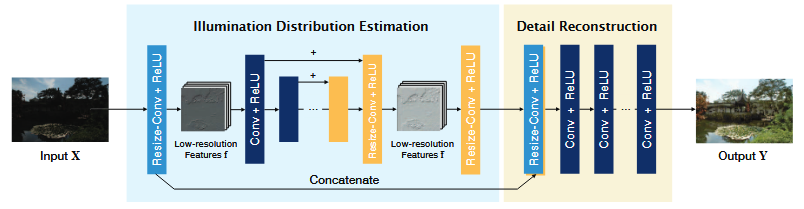
\includegraphics[width=0.8\columnwidth]{GLADNet}
		
		\begin{subfigure}{0.2\textwidth}
			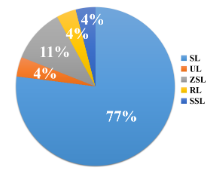
\includegraphics[width=\linewidth]{learning_strategy}
			\captionsetup{font=scriptsize}
			\caption{learning strategy}
			\label{fig:subfig_a}
		\end{subfigure}
		\begin{subfigure}{0.2\textwidth}
			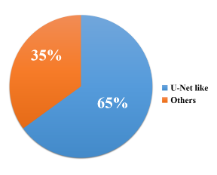
\includegraphics[width=1.15\linewidth]{network_struture}
			\captionsetup{font=scriptsize}
			\caption{network structure}
			\label{fig:subfig_b}
		\end{subfigure}
		\begin{subfigure}{0.2\textwidth}
			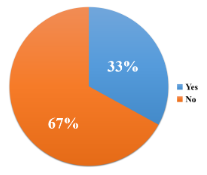
\includegraphics[width=\linewidth]{Retinex_model}
			\captionsetup{font=scriptsize}
			\caption{Retinex model}
			\label{fig:subfig_c}	
		\end{subfigure}
		\begin{subfigure}{0.2\textwidth}
			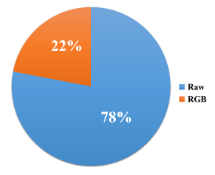
\includegraphics[width=\linewidth]{data_format}
			\captionsetup{font=scriptsize}
			\caption{data format}
			\label{fig:subfig_d}
		\end{subfigure}\\
		\begin{subfigure}{0.2\textwidth}
			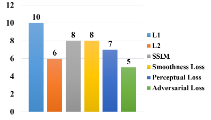
\includegraphics[width=\linewidth]{loss_function}
			\captionsetup{font=scriptsize}
			\caption{loss function}
			\label{fig:subfig_e}
		\end{subfigure}
		\begin{subfigure}{0.2\textwidth}
			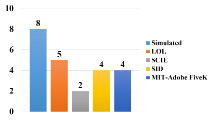
\includegraphics[width=\linewidth]{training_dataset}
			\captionsetup{font=scriptsize}
			\caption{training dataset}
			\label{fig:subfig_f}	
		\end{subfigure}	
		\begin{subfigure}{0.2\textwidth}
			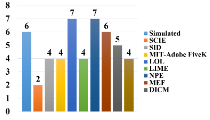
\includegraphics[width=\linewidth]{testing_dataset}
			\captionsetup{font=scriptsize}
			\caption{testing dataset}
			\label{fig:subfig_g}
		\end{subfigure}
		\begin{subfigure}{0.2\textwidth}
			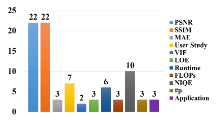
\includegraphics[width=\linewidth]{evaluation_metric}
			\captionsetup{font=scriptsize}
			\caption{evaluation metric}
			\label{fig:subfig_h}	
		\end{subfigure}
		\captionsetup{font=scriptsize}
		\caption{
			\label{fig: Statictic Analysis} % spaces are big no-no withing labels
			% things like fig: are optional in the label but it helps
			% to orient yourself when you have multiple figures,
			% equations and tables
			A statictic analysis of deep learning-based LLIE methods, including learning strategy, network characteristic, Retinex model, data format, loss function, training dataset, testing dataset, and evaluation metric. Better to see with zoom.
		}
	\end{figure}
	
	
	\paragraph{Network Structure} \qquad
	
	从Fig.\ref{fig:subfig_b}可以看来,UNet及类UNet架构占据LLIE的65\%。这是因为:UNet可以有效的集成多尺度特征并同时采用低级与高级特征。这种特性对于取得令人满意的地低光增强非常重要。
	尽管如此,有这样几个问题可能被当前的LLIE网络结构忽略了:
	
	(1) 经过多个卷积层处理后,由于比较小的像素值,极低光图像的梯度可能会在梯度反向传统过程中消失,这可能会导致模型性能并影响网络的收敛;
	
	(2) UNet中的跳过连接可能会引入噪声和冗余特征到最后的结果。如何有效的滤除噪声并同时集成低级与高级特征应该仔细考虑;
	
	(3) 尽管针对LLIE提出了部分设计和成分,但它们往往是从其他相关low-level中修改而来。在设计网络时,低光图像的特征同样应当考虑在内。
	
	
	\paragraph{Combination of Deep Model and Retinex Theory} \qquad
	
	从Fig.\ref{fig:subfig_c}可以看到:近三分之一的方法采用了深度学习+Retinex组合的方式进行设计,采用不同的子网络估计Retinex的不同成分,并估计亮度以引导网络的学习。尽管这种组合可以在深度学习与Retinex之间进行很好的桥接,但可能同时引入各自的弱点到最终的模型:
	
	(1) Retinex的理想假设可能会影响最终的结果;
	
	(2) 深度学习的过拟合可能仍存在;
	
	当组合深度学习与Retinex设计网络时,如何从两者中“取其精华去其糟粕”应该慎重考虑。
	
	
	\paragraph{Data Format} \qquad
	
	正如Fig.\ref{fig:subfig_d}所示,RAW数据是大多数据方法的首选。尽管RAW数据会受限于特定的传感器,但其包含更多的色域以及更高的动态范围。因此,基于RAW数据的深度模型可以重建更清晰的细节、高对比度,具有更好的色彩信息,同时降低了噪声和伪影问题。
	
	尽管如此,由于智能手机的便捷采集性,RGB形式的图像也被不少方法采用并作为输入。在未来的研究中,RAW数据到RGB格式的平滑变化将更有助于LLIE的研究。
	
	
	\paragraph{Loss Function} \qquad
	
	从Fig.\ref{fig:subfig_e}可以看到:LLIE常采用的损失函数为L1, L2, SSIM,感知损失,平滑损失等。除此之外,按照不同的需求,颜色损失、曝光损失、对抗损失同样也得到了应用。
	
	\paragraph{Training Datasets} \qquad
	
	从Fig.\ref{fig:subfig_f}可以看到:不同的成对训练数据被提出并用于LLIE方案的训练。这些数据包含真实数据与合成数据,相关信息见Table \ref{tab: Paired_training_datases}。
	
	\paragraph{Testing Dataset} \qquad
	
		\begin{table}[!htbp]
		\centering
		\tiny
		%\resizebox{\textwidth}{!}{ %按照宽度调整调整表格大小
			\begin{tabular}{>{\centering\arraybackslash}m{2.5cm}|c|c|c|c}

				\hline
				
				\textbf{Name} & \textbf{Number} & \textbf{Format} & \textbf{Real/Syn} & \textbf{Video} \\
				
				\hline
				
				Gamma Correction & $+\infty$ & RGB & Syn & \\
				
				Random Illumination & $+\infty$ & RGB & Syn & \\
				
				\hline
				
				LOL & 500 & RGB & Real & \\
	
				SCIE & 4,413 & RGB & Real & \\
				
				VE-LOL-L & 2,500 & RGB & Real+Syn & \\
				
				MIT-Adobe FiveK & 5,000 & Raw & Real & \\
				
				SID & 5,094 & Raw & Real & \\
				
				DRV & 202 & Raw & Real & \checkmark  \\
				
				SMOID & 179 & Raw & Real & \checkmark  \\
				
				\hline
				
			\end{tabular}
		%}
		\captionsetup{font=scriptsize} %设置标题字体与表格字体一致
		\caption{\label{tab: Paired_training_datases}
			Summary of paired training datasets. 'Syn' represents Synthetic.} %表格的标题
		
	\end{table}
	
	除了上述训练数据集外,还有一些测试数据集,相关信息如Table \ref{tab: Testing datasets}所示。
	
		\begin{table}[!htbp]
		\centering
		\tiny
		%\resizebox{\textwidth}{!}{ %按照宽度调整调整表格大小
			\begin{tabular}{>{\centering\arraybackslash}m{2.5cm}|c|c|c|c}
				
				\hline
				
				\textbf{Name} & \textbf{Number} & \textbf{Format} & \textbf{Application} & \textbf{Video} \\
				
				\hline
				
				LIME & 10 & RGB & &  \\ 
				NPE  & 84 & RGB & &  \\ 
				MEF  & 17 & RGB & &  \\
				DICM & 64 & RGB & &  \\
				 VV  & 24 & RGB & &  \\
				BBD-100K & 10,000 & RGB & \checkmark & \checkmark \\
				ExDARK & 7,363 & RGB & \checkmark & \\ 
				DARK FACE & 6,000 & RGB & \checkmark & \\
				VE-LOL-H & 10,940 & RGB & \checkmark & \\
				
				\hline
				
			\end{tabular}
			%}
		\captionsetup{font=scriptsize} %设置标题字体与表格字体一致
		\caption{\label{tab: Testing datasets}
			Summary of testing datasets.} %表格的标题
		
		\end{table}
	
	\paragraph{Benchmarking and Empirical Analysis} \qquad
	
	在这部分内容中,我们将对现有基于深度学习的LLIE方法进行分析并突出存在的关键挑战。为方便分析,我们提出了一个大尺度低光图像/视频数据以验证不同深度学习方法的性能。除此之外,我们开发了首个在线平台,它包含多种深度学习LLIE方法,用户能够以更友好的交互方式重建不同方法的效果。作者对比的方法有13种,它们分别是:
	
	(1) 监督学习方案:LLNet、LightenNet、Retinex-Net、MBLLEN、KinD、KinD++、TBEFN、DSLR;
	
	(2) 无监督方案:EnlightenGAN;
	
	(3)	半监督方案:DRBN;
	
	(4)	Zero-shot方案:ExCNet、Zero-DCE、RRDNet。
	
	
	\paragraph{A New Low-light Image and Video Dataset} \qquad
	
	作者提出一个大尺度低光图像/视频数据集LoLi-Phone,以进行不同LLIE方案系统而详细的验证对比。LoLi-Phone是目前为止最大的真实低光图像数据。数据与采集设备信息见Table \ref{tab: LoLi-Phone dataset}与Figure 4。
	
		\begin{table}[!htbp]
		\centering
		\tiny
		%\resizebox{\textwidth}{!}{ %按照宽度调整调整表格大小
			\begin{tabular}{>{\centering\arraybackslash}m{2.5cm}|c|c|c}
				
				\hline
				
				\textbf{Phone's Brand} & \textbf{\#Video} & \textbf{\#Image} & \textbf{Resolution} \\
				
				\hline
				
				iPhone 6s   		& 4 & 1,029	& 1920×1080 \\
				iPhone 7 	 		& 13& 6,081 & 1920×1080 \\
				iPhone7 Plus		& 2 & 900   & 1920×1080 \\
				iPhone8 Plus 		& 1 & 489   & 1280×720  \\
				iPhone 11   		& 7 & 2,200 & 1920×1080 \\
				iPhone 11 Pro 		& 17& 7,739 & 1920×1080 \\
				iPhone XS 	 		& 11& 2,470 & 1920×1080 \\
				iPhone XR 			& 16& 4,997 & 1920×1080 \\
				iPhone SE 			& 1 & 455   & 1920×1080 \\
				Xiaomi Mi 9	 		& 2 & 1,145 & 1920×1080 \\
				Xiaomi Mi Mix 3     & 6 & 2,972 & 1920×1080 \\
				Pixel 3   			& 4 & 1,311 & 1920×1080 \\
				Pixel 4   			& 3 & 1,1923& 1920×1080 \\
				Oppo R17 			& 6 & 2,126 & 1920×1080 \\
				Vivo Nex 	 		& 12& 4,097 & 1280×720  \\
				LG M322      		& 2 & 761   & 1920×1080 \\
				OnePlus 5T   		& 1 & 293   & 1920×1080 \\
				Huawei Mate 20 Pro 	& 12& 4,160 & 1920×1080 \\
				
				\hline
				
			\end{tabular}
			%}
		\captionsetup{font=scriptsize} %设置标题字体与表格字体一致
		\caption{\label{tab: LoLi-Phone dataset}
			Summary of LoLi-Phone dataset. LoLi-Phone dataset contains 120 videos (55,148 images) taken by 18 different mobile phones' cameras. "\#Video" and "\#Image" represent the number of videos and images, respectively.} %表格的标题
		
	\end{table}
	
	\begin{figure}[ht] 
		% read manual to see what [ht] means and for other possible options
		\centering 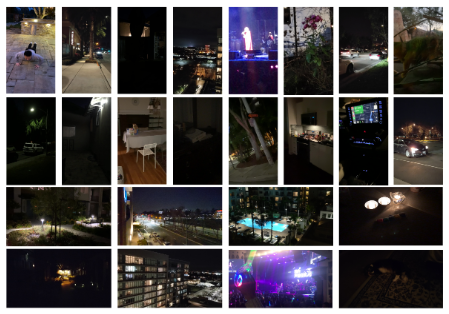
\includegraphics[width=0.8\columnwidth]{Sample_Loli}
		\caption{
			\label{fig:Sample_Loli} % spaces are big no-no withing labels
			% things like fig: are optional in the label but it helps
			% to orient yourself when you have multiple figures,
			% equations and tables
			Several images sampled from the proposed LoLiPhone dataset. The images and videos are taken by different devices under diverse lighting conditions and scenes.
		}
	\end{figure}
	
	\paragraph{Online Evaluation Platform} \qquad
	
	不同方法可能采用不同的深度学习框架,比如Caffe、Theano、TensorFlow以及Pytorch,因此,不同的方法依赖于不同的配置、GPU版本以及硬件信息。这样复杂的需求对于研究员极度不友好,尤其对于出入门者,甚至没有GPU资源的研究员。为缓解该问题,我们开发了在线LLIE平台,称之为LoLi-Platform\footnote{http://mc.nankai.edu.cn/ll/}。
	
	\paragraph{Benchmark Results} \qquad
	
	为更好的定量与定性对比不同的方法,除了LoLi-Phone外,作者还在LOL与MIT-Adboe FiveK数据集上进行了对比。
	
	\begin{figure}[htbp] 
		\centering 
		\begin{subfigure}{0.18\textwidth}
			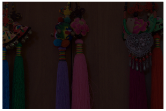
\includegraphics[width=\linewidth]{LOL-test_dataset/input}
			\captionsetup{font=scriptsize}
			\caption{input}
			\label{fig: LOL-test_a}
		\end{subfigure}
		\begin{subfigure}{0.18\textwidth}
			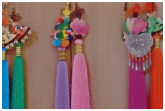
\includegraphics[width=\linewidth]{LOL-test_dataset/LLNet}
			\captionsetup{font=scriptsize}
			\caption{LLNet}
			\label{fig: LOL-test_b}
		\end{subfigure}
		\begin{subfigure}{0.18\textwidth}
			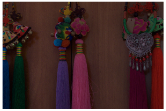
\includegraphics[width=\linewidth]{LOL-test_dataset/LightenNet}
			\captionsetup{font=scriptsize}
			\caption{LightenNet}
			\label{fig: LOL-test_c}  
		\end{subfigure}
		\begin{subfigure}{0.18\textwidth}
			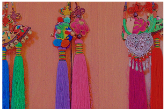
\includegraphics[width=\linewidth]{LOL-test_dataset/Retinex-Net}
			\captionsetup{font=scriptsize}
			\caption{Retinex-Net}
			\label{fig: LOL-test_d}
		\end{subfigure}
		\begin{subfigure}{0.18\textwidth}
			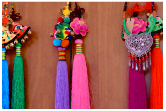
\includegraphics[width=\linewidth]{LOL-test_dataset/MBLLEN}
			\captionsetup{font=scriptsize}
			\caption{MBLLEN}
			\label{fig: LOL-test_e}
		\end{subfigure}\\
		\begin{subfigure}{0.18\textwidth}
			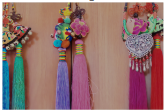
\includegraphics[width=\linewidth]{LOL-test_dataset/KinD}
			\captionsetup{font=scriptsize}
			\caption{KinD}
			\label{fig: LOL-test_f}  
		\end{subfigure}    
		\begin{subfigure}{0.18\textwidth}
			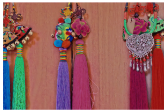
\includegraphics[width=\linewidth]{LOL-test_dataset/KinD++}
			\captionsetup{font=scriptsize}
			\caption{KinD++}
			\label{fig: LOL-test_g}
		\end{subfigure}
		\begin{subfigure}{0.18\textwidth}
			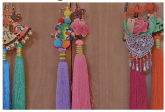
\includegraphics[width=\linewidth]{LOL-test_dataset/TBEFN}
			\captionsetup{font=scriptsize}
			\caption{TBEFN}
			\label{fig: LOL-test_h}  
		\end{subfigure}
		\begin{subfigure}{0.18\textwidth}
			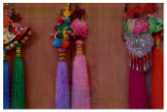
\includegraphics[width=\linewidth]{LOL-test_dataset/DSLR}
			\captionsetup{font=scriptsize}
			\caption{DSLR}
			\label{fig: LOL-test_i}  
		\end{subfigure}
		\begin{subfigure}{0.18\textwidth}
			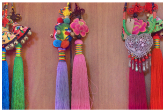
\includegraphics[width=\linewidth]{LOL-test_dataset/EnlightenGAN}
			\captionsetup{font=scriptsize}
			\caption{EnlightenGAN}
			\label{fig: LOL-test_j}  
		\end{subfigure}\\
		\begin{subfigure}{0.18\textwidth}
			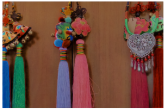
\includegraphics[width=\linewidth]{LOL-test_dataset/DRBN}
			\captionsetup{font=scriptsize}
			\caption{DRBN}
			\label{fig: LOL-test_k}  
		\end{subfigure}    
		\begin{subfigure}{0.18\textwidth}
			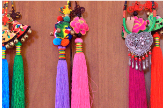
\includegraphics[width=\linewidth]{LOL-test_dataset/ExCNet}
			\captionsetup{font=scriptsize}
			\caption{ExCNet}
			\label{fig: LOL-test_l}
		\end{subfigure}
		\begin{subfigure}{0.18\textwidth}
			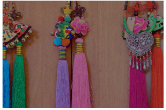
\includegraphics[width=\linewidth]{LOL-test_dataset/Zero-DCE}
			\captionsetup{font=scriptsize}
			\caption{Zero-DCE}
			\label{fig: LOL-test_m}  
		\end{subfigure}
		\begin{subfigure}{0.18\textwidth}
			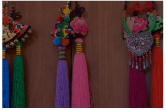
\includegraphics[width=\linewidth]{LOL-test_dataset/RRDNet}
			\captionsetup{font=scriptsize}
			\caption{RRDNet}
			\label{fig: LOL-test_n}  
		\end{subfigure}
		\begin{subfigure}{0.18\textwidth}
			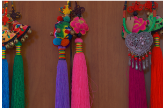
\includegraphics[width=\linewidth]{LOL-test_dataset/GT}
			\captionsetup{font=scriptsize}
			\caption{GT}
			\label{fig: LOL-test_o}  
		\end{subfigure}
		
		\captionsetup{font=scriptsize}
		\caption{
			\label{fig: Visual Result from LOL-test dataset}
			Visual results of different methods on a low-light image sampled from LOL-test dataset.
		}
	\end{figure}
	
	\begin{figure}[htbp] 
		\centering 
		\begin{subfigure}{0.18\textwidth}
			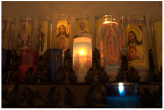
\includegraphics[width=\linewidth]{MIT-Adobe_FiveK/input}
			\captionsetup{font=scriptsize}
			\caption{input}
			\label{fig: MIT-Adobe_FiveK_a}
		\end{subfigure}
		\begin{subfigure}{0.18\textwidth}
			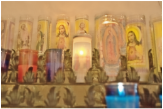
\includegraphics[width=\linewidth]{MIT-Adobe_FiveK/LLNet}
			\captionsetup{font=scriptsize}
			\caption{LLNet}
			\label{fig: MIT-Adobe_FiveK_b}
		\end{subfigure}
		\begin{subfigure}{0.18\textwidth}
			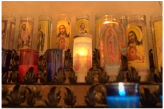
\includegraphics[width=\linewidth]{MIT-Adobe_FiveK/LightenNet}
			\captionsetup{font=scriptsize}
			\caption{LightenNet}
			\label{fig: MIT-Adobe_FiveK_c}  
		\end{subfigure}
		\begin{subfigure}{0.18\textwidth}
			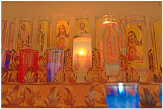
\includegraphics[width=\linewidth]{MIT-Adobe_FiveK/Retinex-Net}
			\captionsetup{font=scriptsize}
			\caption{Retinex-Net}
			\label{fig: MIT-Adobe_FiveK_d}
		\end{subfigure}
		\begin{subfigure}{0.18\textwidth}
			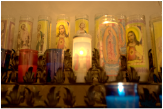
\includegraphics[width=\linewidth]{MIT-Adobe_FiveK/MBLLEN}
			\captionsetup{font=scriptsize}
			\caption{MBLLEN}
			\label{fig: MIT-Adobe_FiveK_e}
		\end{subfigure}\\
		\begin{subfigure}{0.18\textwidth}
			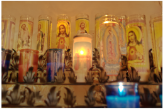
\includegraphics[width=\linewidth]{MIT-Adobe_FiveK/KinD}
			\captionsetup{font=scriptsize}
			\caption{KinD}
			\label{fig: MIT-Adobe_FiveK_f}  
		\end{subfigure}    
		\begin{subfigure}{0.18\textwidth}
			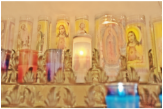
\includegraphics[width=\linewidth]{MIT-Adobe_FiveK/KinD++}
			\captionsetup{font=scriptsize}
			\caption{KinD++}
			\label{fig: MIT-Adobe_FiveK_g}
		\end{subfigure}
		\begin{subfigure}{0.18\textwidth}
			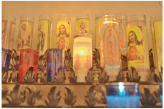
\includegraphics[width=\linewidth]{MIT-Adobe_FiveK/TBEFN}
			\captionsetup{font=scriptsize}
			\caption{TBEFN}
			\label{fig: MIT-Adobe_FiveK_h}  
		\end{subfigure}
		\begin{subfigure}{0.18\textwidth}
			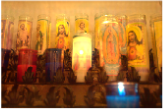
\includegraphics[width=\linewidth]{MIT-Adobe_FiveK/DSLR}
			\captionsetup{font=scriptsize}
			\caption{DSLR}
			\label{fig: MIT-Adobe_FiveK_i}  
		\end{subfigure}
		\begin{subfigure}{0.18\textwidth}
			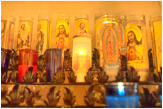
\includegraphics[width=\linewidth]{MIT-Adobe_FiveK/EnlightenGAN}
			\captionsetup{font=scriptsize}
			\caption{EnlightenGAN}
			\label{fig: MIT-Adobe_FiveK_j}  
		\end{subfigure}\\
		\begin{subfigure}{0.18\textwidth}
			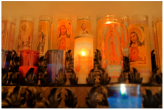
\includegraphics[width=\linewidth]{MIT-Adobe_FiveK/DRBN}
			\captionsetup{font=scriptsize}
			\caption{DRBN}
			\label{fig: MIT-Adobe_FiveK_k}  
		\end{subfigure}    
		\begin{subfigure}{0.18\textwidth}
			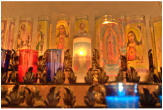
\includegraphics[width=\linewidth]{MIT-Adobe_FiveK/ExCNet}
			\captionsetup{font=scriptsize}
			\caption{ExCNet}
			\label{fig: MIT-Adobe_FiveK_l}
		\end{subfigure}
		\begin{subfigure}{0.18\textwidth}
			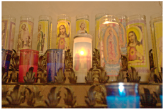
\includegraphics[width=\linewidth]{MIT-Adobe_FiveK/Zero-DCE}
			\captionsetup{font=scriptsize}
			\caption{Zero-DCE}
			\label{fig: MIT-Adobe_FiveK_m}  
		\end{subfigure}
		\begin{subfigure}{0.18\textwidth}
			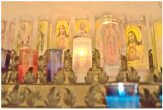
\includegraphics[width=\linewidth]{MIT-Adobe_FiveK/RRDNet}
			\captionsetup{font=scriptsize}
			\caption{RRDNet}
			\label{fig: MIT-Adobe_FiveK_n}  
		\end{subfigure}
		\begin{subfigure}{0.18\textwidth}
			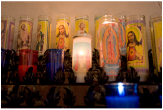
\includegraphics[width=\linewidth]{MIT-Adobe_FiveK/GT}
			\captionsetup{font=scriptsize}
			\caption{GT}
			\label{fig: MIT-Adobe_FiveK_o}  
		\end{subfigure}
		
		\captionsetup{font=scriptsize}
		\caption{
			\label{fig: Visual Result from MIT-Adobe FiveK dataset}
			Visual results of different methods on a low-light image sampled from MIT-Adobe FiveK-test dataset.
		}
	\end{figure}
	
	Fig.\ref{fig: Visual Result from LOL-test dataset}和Fig.\ref{fig: Visual Result from MIT-Adobe FiveK dataset}对比了不同方法在LOL与FiveK数据上的效果对比,可以看到:
	
	在LOL测试数据集上有以下几点发现:
	
	(1) 所有方法均提升了输入图像的亮度和对比,但没有一个能成功进行色彩重建;
	
	(2) LLNet产生了比较的结果;
	
	(3) LightenNet、RRDNet生成欠曝结果,而MBLLEN、ExCNet则生成过曝结果;
	
	(4) KinD、KinD++、TBEFN、DSLR、EnlightenGAN、DRBN则引入明显的伪影;
	
	在FiveK数据集上有以下几点发现:
	
	(1) LLNet、KinD++、TBEFN、RRDNet生成了过曝结果;
	
	(2) Retinex-Net、KinD++、RRDNet生成了伪影,同时又模糊问题。
	
	\begin{figure}[htbp] 
		\centering 
		\begin{subfigure}{0.128\textwidth}
			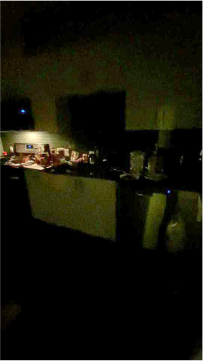
\includegraphics[width=\linewidth]{LoLi-Phone-imgT/input}
			\captionsetup{font=scriptsize}
			\caption{}
			\label{fig: LoLi-Phone-imgT_a}
		\end{subfigure}
		\begin{subfigure}{0.128\textwidth}
			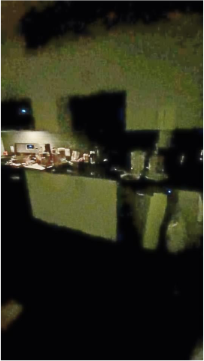
\includegraphics[width=\linewidth]{LoLi-Phone-imgT/LLNet}
			\captionsetup{font=scriptsize}
			\caption{}
			\label{fig: LoLi-Phone-imgT_b}
		\end{subfigure}
		\begin{subfigure}{0.128\textwidth}
			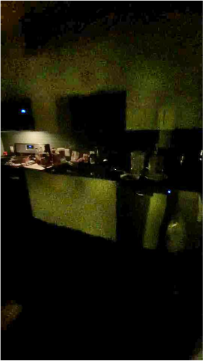
\includegraphics[width=\linewidth]{LoLi-Phone-imgT/LightenNet}
			\captionsetup{font=scriptsize}
			\caption{}
			\label{fig: LoLi-Phone-imgT_c}  
		\end{subfigure}
		\begin{subfigure}{0.128\textwidth}
			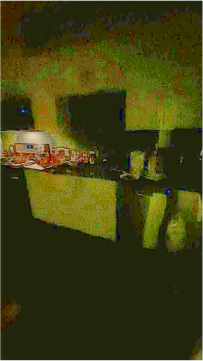
\includegraphics[width=\linewidth]{LoLi-Phone-imgT/Retinex-Net}
			\captionsetup{font=scriptsize}
			\caption{}
			\label{fig: LoLi-Phone-imgT_d}
		\end{subfigure}
		\begin{subfigure}{0.128\textwidth}
			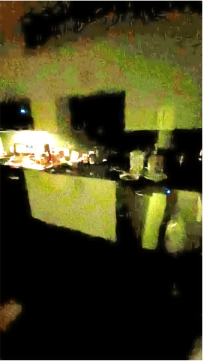
\includegraphics[width=\linewidth]{LoLi-Phone-imgT/MBLLEN}
			\captionsetup{font=scriptsize}
			\caption{}
			\label{fig: LoLi-Phone-imgT_e}
		\end{subfigure}
		\begin{subfigure}{0.128\textwidth}
			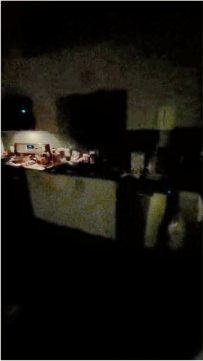
\includegraphics[width=\linewidth]{LoLi-Phone-imgT/KinD}
			\captionsetup{font=scriptsize}
			\caption{}
			\label{fig: LoLi-Phone-imgT_f}  
		\end{subfigure}    
		\begin{subfigure}{0.128\textwidth}
			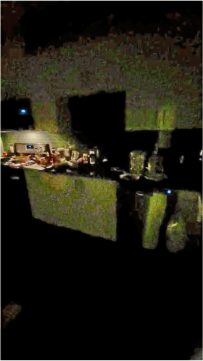
\includegraphics[width=\linewidth]{LoLi-Phone-imgT/KinD++}
			\captionsetup{font=scriptsize}
			\caption{}
			\label{fig: LoLi-Phone-imgT_g}
		\end{subfigure}\\
		\begin{subfigure}{0.128\textwidth}
			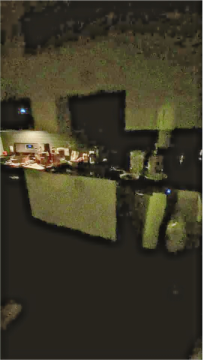
\includegraphics[width=\linewidth]{LoLi-Phone-imgT/TBEFN}
			\captionsetup{font=scriptsize}
			\caption{}
			\label{fig: LoLi-Phone-imgT_h}  
		\end{subfigure}
		\begin{subfigure}{0.128\textwidth}
			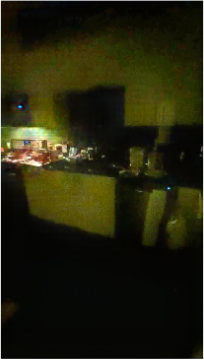
\includegraphics[width=\linewidth]{LoLi-Phone-imgT/DSLR}
			\captionsetup{font=scriptsize}
			\caption{}
			\label{fig: LoLi-Phone-imgT_i}  
		\end{subfigure}
		\begin{subfigure}{0.128\textwidth}
			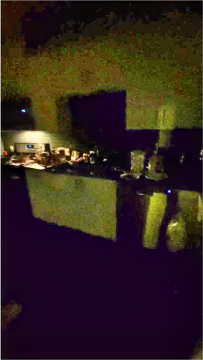
\includegraphics[width=\linewidth]{LoLi-Phone-imgT/EnlightenGAN}
			\captionsetup{font=scriptsize}
			\caption{}
			\label{fig: LoLi-Phone-imgT_j}  
		\end{subfigure}
		\begin{subfigure}{0.128\textwidth}
			\includegraphics[width=\linewidth]{LoLi-Phone-imgT/DRBN}
			\captionsetup{font=scriptsize}
			\caption{}
			\label{fig: LoLi-Phone-imgT_k}  
		\end{subfigure}    
		\begin{subfigure}{0.128\textwidth}
			\includegraphics[width=\linewidth]{LoLi-Phone-imgT/ExCNet}
			\captionsetup{font=scriptsize}
			\caption{}
			\label{fig: LoLi-Phone-imgT_l}
		\end{subfigure}
		\begin{subfigure}{0.128\textwidth}
			\includegraphics[width=\linewidth]{LoLi-Phone-imgT/Zero-DCE}
			\captionsetup{font=scriptsize}
			\caption{}
			\label{fig: LoLi-Phone-imgT_m}  
		\end{subfigure}
		\begin{subfigure}{0.128\textwidth}
			\includegraphics[width=\linewidth]{LoLi-Phone-imgT/RRDNet}
			\captionsetup{font=scriptsize}
			\caption{}
			\label{fig: LoLi-Phone-imgT_n}  
		\end{subfigure}\\
		
		\captionsetup{font=scriptsize}
		\caption{
			\label{fig: Visual Result from LoLi-Phone-imgT dataset}
			Visual results of different methods on a low-light image sampled from LoLi-Phone-imgT dataset. (a) input (b) LLNet (c) LightenNet (d) Retinex-Net (e) MBLLEN  (f) KinD  (g) KinD++  (h) TBEFN  (i) DSLR  (j) EnlightenGAN  (k) DRBN  (l) ExCNet  (m) Zero-DCE  (n) RRDNet 
		}
	\end{figure}
	
	
	\begin{figure}[htbp] 
		\centering 
		\begin{subfigure}{0.128\textwidth}
			\includegraphics[width=\linewidth]{LoLi-Phone-imgT_1/input}
			\captionsetup{font=scriptsize}
			\caption{}
			\label{fig: LoLi-Phone-imgT_1_a}
		\end{subfigure}
		\begin{subfigure}{0.128\textwidth}
			\includegraphics[width=\linewidth]{LoLi-Phone-imgT_1/LLNet}
			\captionsetup{font=scriptsize}
			\caption{}
			\label{fig: LoLi-Phone-imgT_1_b}
		\end{subfigure}
		\begin{subfigure}{0.128\textwidth}
			\includegraphics[width=\linewidth]{LoLi-Phone-imgT_1/LightenNet}
			\captionsetup{font=scriptsize}
			\caption{}
			\label{fig: LoLi-Phone-imgT_1_c}  
		\end{subfigure}
		\begin{subfigure}{0.128\textwidth}
			\includegraphics[width=\linewidth]{LoLi-Phone-imgT_1/Retinex-Net}
			\captionsetup{font=scriptsize}
			\caption{}
			\label{fig: LoLi-Phone-imgT_1_d}
		\end{subfigure}
		\begin{subfigure}{0.128\textwidth}
			\includegraphics[width=\linewidth]{LoLi-Phone-imgT_1/MBLLEN}
			\captionsetup{font=scriptsize}
			\caption{}
			\label{fig: LoLi-Phone-imgT_1_e}
		\end{subfigure}
		\begin{subfigure}{0.128\textwidth}
			\includegraphics[width=\linewidth]{LoLi-Phone-imgT_1/KinD}
			\captionsetup{font=scriptsize}
			\caption{}
			\label{fig: LoLi-Phone-imgT_1_f}  
		\end{subfigure}    
		\begin{subfigure}{0.128\textwidth}
			\includegraphics[width=\linewidth]{LoLi-Phone-imgT_1/KinD++}
			\captionsetup{font=scriptsize}
			\caption{}
			\label{fig: LoLi-Phone-imgT_1_g}
		\end{subfigure}\\
		\begin{subfigure}{0.128\textwidth}
			\includegraphics[width=\linewidth]{LoLi-Phone-imgT_1/TBEFN}
			\captionsetup{font=scriptsize}
			\caption{}
			\label{fig: LoLi-Phone-imgT_1_h}  
		\end{subfigure}
		\begin{subfigure}{0.128\textwidth}
			\includegraphics[width=\linewidth]{LoLi-Phone-imgT_1/DSLR}
			\captionsetup{font=scriptsize}
			\caption{}
			\label{fig: LoLi-Phone-imgT_1_i}  
		\end{subfigure}
		\begin{subfigure}{0.128\textwidth}
			\includegraphics[width=\linewidth]{LoLi-Phone-imgT_1/EnlightenGAN}
			\captionsetup{font=scriptsize}
			\caption{}
			\label{fig: LoLi-Phone-imgT_1_j}  
		\end{subfigure}
		\begin{subfigure}{0.128\textwidth}
			\includegraphics[width=\linewidth]{LoLi-Phone-imgT_1/DRBN}
			\captionsetup{font=scriptsize}
			\caption{}
			\label{fig: LoLi-Phone-imgT_1_k}  
		\end{subfigure}    
		\begin{subfigure}{0.128\textwidth}
			\includegraphics[width=\linewidth]{LoLi-Phone-imgT_1/ExCNet}
			\captionsetup{font=scriptsize}
			\caption{}
			\label{fig: LoLi-Phone-imgT_1_l}
		\end{subfigure}
		\begin{subfigure}{0.128\textwidth}
			\includegraphics[width=\linewidth]{LoLi-Phone-imgT_1/Zero-DCE}
			\captionsetup{font=scriptsize}
			\caption{}
			\label{fig: LoLi-Phone-imgT_1_m}  
		\end{subfigure}
		\begin{subfigure}{0.128\textwidth}
			\includegraphics[width=\linewidth]{LoLi-Phone-imgT_1/RRDNet}
			\captionsetup{font=scriptsize}
			\caption{}
			\label{fig: LoLi-Phone-imgT_1_n}  
		\end{subfigure}\\
		
		\captionsetup{font=scriptsize}
		\caption{
			\label{fig: Visual Result from LoLi-Phone-imgT_1 dataset}
			Visual results of different methods on a low-light image sampled from LoLi-Phone-imgT dataset. (a) input (b) LLNet (c) LightenNet (d) Retinex-Net (e) MBLLEN  (f) KinD  (g) KinD++  (h) TBEFN  (i) DSLR  (j) EnlightenGAN  (k) DRBN  (l) ExCNet  (m) Zero-DCE  (n) RRDNet 
		}
	\end{figure}
	
	Fig.\ref{fig: Visual Result from LoLi-Phone-imgT dataset} 和Fig.\ref{fig: Visual Result from LoLi-Phone-imgT_1 dataset}给出了LoLi-Phone数据集上的效果对比,可以看到:
	
	对于Fig.\ref{fig: Visual Result from LoLi-Phone-imgT dataset}有以下几点发现:
	
	(1) 所有方法均无法有效改进亮度并移除噪声;
	
	(2) Retinex-Net、MBLLEN、DRBN生成了明显伪影;
	
	对于和Fig.\ref{fig: Visual Result from LoLi-Phone-imgT_1 dataset}有以下几点发现:
	
	(1) 所有方法均增强了输入图像的亮度;
	
	(2) 仅有MBLLEN、RRDNet取得视觉友好的增强效果,且无色片、伪影以及欠/过曝问题。
	
	
	\begin{table}[!htbp]
		\centering
		\tiny
		\resizebox{\textwidth}{!}{ %按照宽度调整调整表格大小
			\begin{tabular}{>{\centering\arraybackslash}m{2cm}|>{\centering\arraybackslash}m{2.5cm}|c|c|c|c|c|c|c|c}
				
				\hline %添加表格头部粗线
				
				% \multirow{2}*{\textbf{Learning}} & \multirow{2}*{\textbf{Mathod}} & \multicolumn{4}{c|}{\textbf{LOL-test}} & \multicolumn{4}{c}{\textbf{MIT-Adobe FiveK-test}} \\
				
				\multirowcell{2}{\centering\textbf{Learning}} & \multirowcell{2}{\textbf{Method}} & \multicolumn{4}{c|}{\makecell{\textbf{LOL-test}}} & \multicolumn{4}{c}{\makecell{\textbf{MIT-Adobe FiveK-test}}} \\
				
				\cline{3-10}
				
				
				& 		 & \textbf{MSE↓}  & \textbf{PSNR↑} & \textbf{SSIM↑} & \textbf{LPIPS↓} & \textbf{MSE↓}  & \textbf{PSNR↑}  & \textbf{SSIM↑} & \textbf{LPIPS↓} \\
				
				\hline
				
				& input & 12.613& 7.773 & 0.181 & 0.560  & 1.670 & 17.824 & 0.779 & 0.148  \\
				
				\hline	
				
				\multirowcell{8}{SL} & LLNet & 1.290 & 17.959& 0.713 & 0.360  & 4.465 & 12.177 & 0.645 & 0.292 \\
				& LightenNet & 7.614 & 10.301& 0.402 & 0.394  & 4.127 & 13.579 & 0.744 & 0.166 \\
				& Retinex-Net& 1.651 & 16.774& 0.462 & 0.474  & 4.406 & 12.310 & 0.671 & 0.239 \\
				& MBLLEN 	 & 1.444 & 17.902& 0.715 & 0.247  &	1.296 & 19.781 & 0.825 & 0.108 \\
				& KinD 		 & 1.431 & 17.648& 0.779 & 0.175  & 2.675 & 14.535 & 0.741 & 0.177 \\
				& KinD++     & 1.298 & 17.752& 0.760 & 0.198  & 7.582 & 9.732  & 0.568 & 0.336 \\
				& TBEFN 	 & 1.764 & 17.351& 0.786 & 0.210  & 3.865 & 12.769 & 0.704 & 0.178 \\
				& DSLR 		 & 3.536 & 15.050& 0.597 & 0.337  & 1.925 & 16.632 & 0.782 & 0.167 \\
				
				\hline
				
				UL & EnlightenGAN & 1.998 & 17.483& 0.677 & 0.322  & 3.628 & 13.260 & 0.745 & 0.170 \\
				
				\hline
				
				SSL  & DRBN       & 2.359 & 15.125& 0.472 & 0.316  & 3.314 & 13.355 & 0.378 & 0.281 \\ 
				
				\hline
				
				\multirowcell{3}{ZSL} & ExCNet&2.292 & 15.783& 0.515 & 0.373  & 2.927 & 13.978 & 0.710 0.187   \\
				& Zero-DCE 	 & 3.282 & 14.861& 0.589 & 0.335  & 3.476 & 13.199 & 0.709 0.203   \\
				& RRDNet     & 6.313 & 11.392& 0.468 & 0.361  & 7.057 & 10.135 & 0.620 0.303   \\
				
				
				\hline
				
			\end{tabular}
		}
		\captionsetup{font=scriptsize} %设置标题字体与表格字体一致
		\caption{\label{tab: Quantitative Comparisons on LOL-test and MIT-Adobe FiveK-test testing datasets}
			Quantitative comparisons on LOL-test and MIT-Adobe FiveK-test testing datasets in terms of MSE (×103), PSNR (in dB), SSIM, and LPIPS. The best result is in red whereas the second and third best results are in blue and purple under each case, respectively.} %表格的标题
		
	\end{table}
	
	\begin{table}[!htbp]
		\centering
		\tiny
		% \resizebox{\textwidth}{!}{ %按照宽度调整调整表格大小
			\begin{tabular}{>{\centering\arraybackslash}m{2cm}|>{\centering\arraybackslash}m{2.5cm}|c|c|c|c}
				
				\hline %添加表格头部粗线
				
				% \multirow{2}*{\textbf{Learning}} & \multirow{2}*{\textbf{Mathod}} & \multicolumn{4}{c|}{\textbf{LOL-test}} & \multicolumn{4}{c}{\textbf{MIT-Adobe FiveK-test}} \\
				
				\multirowcell{2}{\centering\textbf{Learning}} & \multirowcell{2}{\textbf{Method}} & \multicolumn{4}{c}{\makecell{\textbf{LoLi-Phone-imgT}}}  \\
				
				\cline{3-6}
				
				
				& 		 & \textbf{NIQE↓}  & \textbf{LOE↓} & \textbf{PI↓} & \textbf{SPAQ↑} \\
				
				\hline
				
				& input & 6.99 & \textcolor{red}{0.00} & 5.86 & 44.45 \\
				
				\hline	
				
				\multirowcell{8}{SL} & LLNet & 5.86  & \textcolor{blue}{5.86}   & 5.66 & 40.56   \\
				& LightenNet & 5.34  & 952.33 & 4.58 & 45.74   \\
				& Retinex-Net& 5.01  & 790.21 & \textcolor{red}{3.48} & \textcolor{red}{50.95}   \\
				& MBLLEN 	 & 5.08  & 220.63 & 4.27 & 42.50   \\
				& KinD 		 & 4.97  & 405.88 & 4.37 & 44.79   \\
				& KinD++     & \textcolor{red}{4.73}  & 681.97 & \textcolor{blue}{3.99} & \textcolor{blue}{46.89}   \\
				& TBEFN 	 & 4.81  & 552.91 & 4.30 & 44.14   \\
				& DSLR 		 & \textcolor{blue}{4.77}  & 447.98 & 4.31 & 41.08   \\
				
				\hline
				
				UL & EnlightenGAN & \textcolor{red}{4.79}  & 821.87 & \textcolor{red}{4.19} & 45.48   \\
				
				\hline
				
				SSL  & DRBN       & 5.80  & 885.75 & 5.54 & 42.74   \\ 
				
				\hline
				
				\multirowcell{3}{ZSL}& ExCNet& 5.55 & 723.56 & 4.38 & 46.74   \\
				& Zero-DCE& 5.82 & 307.09 & 4.76 & \textcolor{red}{46.85}   \\
				& RRDNet  & 5.97 & \textcolor{red}{142.89} & 4.84 & 45.31   \\
				
				
				\hline
				
			\end{tabular}
			% }
		\captionsetup{font=scriptsize} %设置标题字体与表格字体一致
		\caption{\label{tab: Quantitative comparisons on LoLi-Phone-imgT dataset}
			Quantitative comparisons on LoLi-Phone-imgT dataset in terms of NIQE, LOE, PI, and SPAQ. The best result is in red whereas the second and third best results are in blue and purple under each case, respectively.} %表格的标题
		
	\end{table}
	
	Table \ref{tab: Quantitative Comparisons on LOL-test and MIT-Adobe FiveK-test testing datasets}给出了不同方法在LOL与FiveK数据上的定量指标对比,可以看到:
	
	
	(1) 有监督方案具有更高的指标;
	
	(2) LLNet在LOL-test数据上取得了最佳MSE与PSNR;
	
	(3) TBEFN在LOL-test数据上取得了最佳SSIM指标;
	
	(4) KinD在LOL-test数据上取得了最佳LPIPS指标;	
	
	(5)对于FiveK-test数据,MBLLEN取得了全面性的指标优先。
	
	
	Table \ref{tab: Quantitative comparisons on LoLi-Phone-imgT dataset}对比了不同方法在LoLi-Phone-imgT数据上的指标对比,可以看到:
	
	(1) Retinex-Net、KinD++、EnlightenGAN具有相对更佳的性能;
	
	(2) Retinex-Net取得了最佳PI与SPAQ指标,然而从视觉效果上看,它仍存在伪影和色偏问题;
	
	(3) KinD++取得了最佳NIQE指标。
	
	\paragraph{Computational Complexity} \qquad
	
	\begin{table}[!htbp]
		\centering
		\tiny
		% \resizebox{\textwidth}{!}{ %按照宽度调整调整表格大小
			\begin{tabular}{>{\centering\arraybackslash}m{1.5cm}|>{\centering\arraybackslash}m{2.5cm}|c|c|c|c}
				
				\hline %添加表格头部粗线
				
				% \multirow{2}*{\textbf{Learning}} & \multirow{2}*{\textbf{Mathod}} & \multicolumn{4}{c|}{\textbf{LOL-test}} & \multicolumn{4}{c}{\textbf{MIT-Adobe FiveK-test}} \\
				
				\textbf{Learning} & \textbf{Method} & \textbf{RunTime↓} & \textbf{\#Parameters↓} & \textbf{FLOPs↓} & \textbf{Platform} \\
				
				\hline	
				
				\multirowcell{8}{SL} & LLNet & 36.270 & 17.908 & 4124.177 & Theano   \\
				& LightenNet & - & \textcolor{red}{0.030} & \textcolor{red}{30.540} & MATLAB   \\
				& Retinex-Net& 0.120 & 0.555 & 587.470 & TensorFlow  \\
				& MBLLEN 	 & 13.995 & \textcolor{purple}{0.450} & 301.120 & TensorFlow   \\
				& KinD 		 & 0.148 & 8.160 & 574.954 & TensorFlow   \\
				& KinD++     & 1.068 & 8.275 & 12238.026 & TensorFlow   \\
				& TBEFN 	 & \textcolor{purple}{0.050} &  0.486 & 108.532 & TensorFlow   \\
				& DSLR 		 & 0.074 &14.931 & \textcolor{purple}{96.683} & PyTorch   \\
				
				\hline
				
				UL & EnlightenGAN & \textcolor{blue}{0.008} & 8.637 & 273.240 & PyTorch   \\
				
				\hline
				
				SSL  & DRBN       & 0.878 & 0.577 & 196.359 & PyTorch   \\ 
				
				\hline
				
				\multirowcell{3}{ZSL}& ExCNet& 23.280 & 8.274 & - & PyTorch   \\
				& Zero-DCE& \textcolor{red}{0.003} & \textcolor{blue}{0.079} & \textcolor{blue}{84.990} & PyTorch   \\
				& RRDNet  & 167.260 & 0.128 & - & PyTorch   \\
				
				
				\hline
				
			\end{tabular}
			% }
		\captionsetup{font=scriptsize} %设置标题字体与表格字体一致
		\caption{\label{tab: Quantitative comparisons of computational complexity}
			Quantitative comparisons of computational complexity in terms of runtime (in second), number of trainable parameters (\#Parameters) (in M), and FLOPs (in G). The best result is in \textcolor{red}{red} whereas the second and third best results are in \textcolor{blue}{blue} and \textcolor{purple}{purple} under each case, respectively. ‘-’ indicates the result is not available.} %表格的标题
	\end{table}
	
	Table \ref{tab: Quantitative comparisons of computational complexity}对比了不同方法的计算复杂度、参数量以及耗时对比。从中可以看到:
	
	(1) Zero-DCE具有最快的推理速度;相反,ExCNet与RRDNet具有最长的推理耗时;
	
	(2) LightenNet具有最少的可学习参数量;相反,LLNet与KinD++的计算量分别高达
	4124.18G与12238.03G。
	
	
	\paragraph{Application-based Evaluation} \qquad
	
	\begin{figure}[ht] 
		% read manual to see what [ht] means and for other possible options
		\centering \includegraphics[width=0.8\columnwidth]{P-R_curves}
		\captionsetup{font=scriptsize}
		\caption{
			\label{fig: P-R_curves} % spaces are big no-no withing labels
			% things like fig: are optional in the label but it helps
			% to orient yourself when you have multiple figures,
			% equations and tables
			The P-R curves of face detection in the dark.
		}
	\end{figure}
	
		\begin{figure}[htbp] 
		\centering 
		\begin{subfigure}{0.22\textwidth}
			\includegraphics[width=\linewidth]{DARK_FACE/input}
			\captionsetup{font=scriptsize}
			\caption{input}
			\label{fig: DARK_FACE_a}
		\end{subfigure}
		\begin{subfigure}{0.22\textwidth}
			\includegraphics[width=\linewidth]{DARK_FACE/LightenNet}
			\captionsetup{font=scriptsize}
			\caption{LightenNet}
			\label{fig: DARK_FACE_b}
		\end{subfigure}
		\begin{subfigure}{0.22\textwidth}
			\includegraphics[width=\linewidth]{DARK_FACE/Retinex-Net}
			\captionsetup{font=scriptsize}
			\caption{Retinex-Net}
			\label{fig: DARK_FACE_c}
		\end{subfigure}
		\begin{subfigure}{0.22\textwidth}
			\includegraphics[width=\linewidth]{DARK_FACE/MBLLEN}
			\captionsetup{font=scriptsize}
			\caption{MBLLEN}
			\label{fig: DARK_FACE_d}
		\end{subfigure}\\ 
		\begin{subfigure}{0.22\textwidth}
			\includegraphics[width=\linewidth]{DARK_FACE/KinD++}
			\captionsetup{font=scriptsize}
			\caption{KinD++}
			\label{fig: DARK_FACE_e}
		\end{subfigure}
		\begin{subfigure}{0.22\textwidth}
			\includegraphics[width=\linewidth]{DARK_FACE/TBEFN}
			\captionsetup{font=scriptsize}
			\caption{TBEFN}
			\label{fig: DARK_FACE_f}  
		\end{subfigure}
		\begin{subfigure}{0.22\textwidth}
			\includegraphics[width=\linewidth]{DARK_FACE/DSLR}
			\captionsetup{font=scriptsize}
			\caption{DSLR}
			\label{fig: DARK_FACE_g}  
		\end{subfigure}
		\begin{subfigure}{0.22\textwidth}
			\includegraphics[width=\linewidth]{DARK_FACE/EnlightenGAN}
			\captionsetup{font=scriptsize}
			\caption{EnlightenGAN}
			\label{fig: DARK_FACE_h}  
		\end{subfigure}\\
		\begin{subfigure}{0.22\textwidth}
			\includegraphics[width=\linewidth]{DARK_FACE/DRBN}
			\captionsetup{font=scriptsize}
			\caption{DRBN}
			\label{fig:DARK_FACE_i}  
		\end{subfigure}    
		\begin{subfigure}{0.22\textwidth}
			\includegraphics[width=\linewidth]{DARK_FACE/ExCNet}
			\captionsetup{font=scriptsize}
			\caption{ExCNet}
			\label{fig: DARK_FACE_j}
		\end{subfigure}
		\begin{subfigure}{0.22\textwidth}
			\includegraphics[width=\linewidth]{DARK_FACE/Zero-DCE}
			\captionsetup{font=scriptsize}
			\caption{Zero-DCE}
			\label{fig: DARK_FACE_k}  
		\end{subfigure}
		\begin{subfigure}{0.22\textwidth}
			\includegraphics[width=\linewidth]{DARK_FACE/RRDNet}
			\captionsetup{font=scriptsize}
			\caption{RRDNet}
			\label{fig: DARK_FACE_l}  
		\end{subfigure}
		
		\captionsetup{font=scriptsize}
		\caption{
			\label{fig: Visual Result from DARK_FACE dataset}
			Visual results of different methods on a low-light image sampled from DARK FACE dataset. Better see with zoom in for the bounding boxes of faces.
		}
	\end{figure}
	
	Fig.\ref{fig: P-R_curves}与Fig.\ref{fig: Visual Result from DARK_FACE dataset}给出了任务相关的质量评价与视觉效果对比。可以看到:\textbf{所有方案均可以改善低光场景下的人脸检测}。
	
	\paragraph{Discussion} \qquad
	
	从上述实验结果,我们可以得到以下几点有意思发现与洞见:
	
	(1) 在不同测试集、不同评估准则上,不同方法的性能变大非常大。在全参考IQA评估+通用测试数据上,MBLLEN、KinD++、DSLR表象更佳;在真实低光场景,Retinex-Net、KinD++去更好的无参考IQA得分;TBEFN具有更好的时序一致性;当考虑计算效率时,Zero-DCE表现最为突出;从人脸检测角度看,TBEFN、Retinex-Net、Zero-DCE排前三。总而言之,Retinex-Net、Zero-DCE、DSLR最大多数场景的更佳选择。
	
	(2) 大多数方法在面对LoLi-Phone时出现失败现象,也就是说现有方案的泛化性能需要进一步改善。
	
	(3) 从学习策略来看,监督学习可以取得更佳性能,但需要高计算资源与成对数据;相反,在真实场景,zero-shot学习更令人期待。
	
	(4) 在视觉效果与量化IQA指标方面存在明显的gap,也就是说:好的视觉效果并不总是具有好的IQA得分。
	
	(5)基于深度学习的LLIE方法有助于低光人脸检测性能提升。
	
	
	
	
	\paragraph{Future Research Directions}
	
	尽管LLIE取得极大的进展,但仍有改善的空间。作者从以下几个方面提出了有价值的参考:	
		
		\subparagraph{Effective Learning Strategies}
		
		当前主流的监督学习方法需要大量的成对训练数据,且可能导致特定数据过拟合问题;Zero-shot学习在真实场景具有更强的鲁棒性,且不需要成对训练数据。这意味着:Zero-shot学习是一个极具潜力的研究方向。
			
		\subparagraph{Specialized Network Structures}
		
		网络结构可以很大程度影响增强性能,之前的LLIE方案大量的采用了UNet架构,然而这种架构是否适合于LLIE仍有待于考证。局部自相似性、高效算子、NAS技术等思想可以考虑引入到LLIE的网络脚骨设计中,此外transformer也许会是一个有意思的研究方向。
		
		\subparagraph{Loss Function}
		
		损失函数约束了输入与GT之间的相关性并驱动网络的优化。在LLIE中,常用损失函数主要是从其他相关任务中借鉴而来,尚未有针对LLIE而设计的特定损失。更适合LLIE的损失函数设计仍有待于开发。
		
		\subparagraph{Realistic Training Data}
		
		尽管已有不少用于LLIE的训练数据,但它们数量、灵活性相对于真实低光比较单一且简单。大尺度的真实LLIE数据收集与生成仍需要进一步研究。
		
		\subparagraph{Standard Testing Data}
		
		目前没有一个可以全面接受的LLIE评估基准。研究员倾向于使用自有测试集,这使得所提方法具有一定倾向性。因此,高质量标准低光图像/视频测试集的构建需要进行构建。
		
		\subparagraph{Task-Specific Evaluation Metrics}
		
		在某种程度上,常用的度量准则难以很好的反映图像质量。如何评价LLIE增强结果的好坏仍极具挑战,当前IQA要么聚焦于人类视觉感知,要么聚焦机器感知。同时考虑人类视觉感知与机器感知的度量指标有待于开发。
		
		\subparagraph{Robust Generalization Capability}
		
		实验结果表明:现有方法在真实场景表现差强人意。这种泛化性能差主要有这样几个因素:合成数据、小尺度训练数据、低效网络结构、不真实的假设、不精确的先验。因此,很有必要探索更好的方式改善LLIE的泛化性能。
		
		\subparagraph{Extension to Low-light Video Enhancement}
		
		不同于其他low-level领域视频增强(比如视频去模糊、视频降噪、视频超分)的快速发展,低光视频增强鲜少收到关注。低光图像增强的直接应用会导致不令人满意的结果与抖动问题。因此,如何采用近邻帧有效移除视觉抖动并加速推理值得深入研究。
		
		\subparagraph{Integrating Semantic Information}
		
		语义信息对于低光增强非常重要,它将引导网络判别不同区域的增处理。如何有效地将语义信息集成到低光增强是一个有前途的方向。
	
	
	\subsubsection{项目链接}
	
	该综述所提出的数据集以及在线平台可以作为进一步研究的参考资源,并促进该领域的进一步发展。所提平台与所收集的算法、数据集、评估准则等等均已公开到GitHub\footnote{https://github.com/Li-Chongyi/Lighting-the-Darkness-in-the-Deep-Learning-Era-Open.
	}。
	
	\subsection{GLADNet: Low Light Enhancement Network with Global Awareness}
	
	GLADNet\cite{GLADNet}的核心:(1)为低光输入计算全局亮度估计;(2)基于前述所得与原始输入调整亮度。它将输入图像缩放到特定尺寸并送入到编解码网络中生成关于亮度的全局先验信息,基于全局先验信息与原始输入图像,采用卷积神经网络进行细节还原。在训练过程中,作者采用RAW图像合成的数据进行训练。通过大量实验验证了所提方法的有效性。
	
	\begin{figure}[ht] 
		% read manual to see what [ht] means and for other possible options
		\centering \includegraphics[width=0.8\columnwidth]{GLADNet}
		\caption{
			\label{fig:GLADNet} % spaces are big no-no withing labels
			% things like fig: are optional in the label but it helps
			% to orient yourself when you have multiple figures,
			% equations and tables
			The architecture of GLADNet. The architecture consists of two steps, global illumination estimation step and detail reconstruction step. In the first step, the encoder-decoder network produces an illumination estimation of a fixed size (96 × 96 here). In the second step, a convolutional network utilizes the input image and the outputs from the previous step to compensate the details.
		}
	\end{figure}
	
 	Fig.\ref{fig:GLADNet}给出GLADNet的框架图,从中可以看出,该网络由两部分构成:全局亮度先验估计和细节还原。
	
	\subsubsection{全局亮度先验估计}
	
	在该部分中,作者采用了一个编解码网络架构用于估计全局亮度信息。注:为估计亮度信息,它需要将输入图像下采样到固定尺寸,这样可以保证该架构的底层感受野可以包含整个图像。
	该子网络包含三个步骤:(1)缩放输入特征到特定分辨率$96\times96$;(2) 采用编解码架构估计全局亮度信息;(3) 缩放到原始分辨率。
	
	\subsubsection{细节还原}	
	
	全局亮度估计过程中由于尺度缩放问题会导致细节损失,为弥补该问题,作者设计了该细节还原子网络。
	
	相比编解码网络输出,原始输入图像应当包含更多的细节信息,因而可以为细节还原提供更多信息。该子网络以全局亮度信息+原始输入图像作为输入(这样可以保证了原始信息与亮度估计互补并传递到后续网络),该子网络另外包含三个卷积操作。
	
	\subsubsection{损失函数}
	
	作者在训练过程中采用RAW图像进行训练数据的合成,采用加权$L_1$损失函数进行训练。加权$L_1$损失函数定义如下:
	\begin{equation}\label{eq:L1} % the label is used to reference the equation
	Loss\left(X,Y\right)=\frac{1}{N}\sum_{i}^{N}\sum_{c=r,g,b}\lambda_{c}{\left \|F(X_i,\theta)^{c}-Y_{i}^c \right\|}_{1},
	\end{equation}
	其中,$\lambda_r=0.29891,\ \lambda_g=0.58661,\ \lambda_b=0.1148$,这种参数设置可以保证颜色平衡问题,提升网络的鲁棒性。

	
	\subsection{Deep Retinex Decomposition for Low Light Enhancement}

	Retinex是一种有效的低光图像增强方法。它假设观测图像可以被分解为Reflectance
	与Illumination。现有的基于Retinex的模型需要精心设计人工约束条件与参数用于求解该病态分解问题(这限制了模型在不同场景应用中的泛化性能)。
	
	作者收集了一批低亮度图像对(含低光与正常光图像)并提出一种RetinexNet架构在该数据集上进行训练学习。RetinexNet包含一个DecomNet用于图像分解分解以及一个Enha-nceNet用于亮度调整。在训练过程中,DeconmNet并没有关于Reflectance与Illumination的真值。因而,该网络学习了这样的关键约束:图像对的反射一致性与亮度的平滑一致性。基于该分解方案,EnhanceNet用来进行亮度增强,同时需要对Reflectance进行降噪处理。该RetinexNet可以通过端到端的方式进行训练。
	
	大量实验表明:RetinexNet不仅取得极好的视觉效果,同时可以提供一种良好的图像分解表达。
	
	RetinexNet\footnote{注:为训练这样一个网络,作者利用RAW数据集构建了一个包含真实与合成图像的低光数据集。}是一种数据驱动的Retinex分解方法,它集成图像分解与增强操作于一体。如Fig.\ref{fig:RetinexNet}给出RetinexNet的框架图,分为如下三个步骤。
	
	\begin{figure}[ht] 
		% read manual to see what [ht] means and for other possible options
		\centering \includegraphics[width=0.8\columnwidth]{RetinexNet}
		\caption{
			\label{fig:RetinexNet} % spaces are big no-no withing labels
			% things like fig: are optional in the label but it helps
			% to orient yourself when you have multiple figures,
			% equations and tables
			The proposed framework for Retinex-Net. The enhancement process is divided into three steps: decomposition, adjustment and reconstruction. In the decomposition step, a subnetwork Decom-Net decomposes the input image into reflectance and illumination. In the following adjustment step, an encoder-decoder based Enhance-Net brightens up the illumination. Multi-scale concatenation is introduced to adjust the illumination from multi-scale perspectives. Noise on the reflectance is also removed at this step. Finally, we reconstruct the adjusted illumination and reflectance to get the enhanced result.
		}
	\end{figure}
	
	首先,子网络DecomNet用于将观测图像划分为亮度独立的反射图与结构平滑的亮度图;
	DecomNet网络存在两个约束条件:(1) 低光与正常光具有相同的反射图;(2) 亮度图应该是平滑的且保留有主要结构(可通过结构相关的全变差损失约束学习)。
	在训练过程中,它以成对图像作为输入(用于约束反射一致性);在测试阶段仅需要输入低光图像。
	
	然后,子网络EnhanceNet通过多尺度Concat操作调整亮度图以保证(1)在大范围内保持一致;(2)小范围内进行裁剪局部分布。
	它主要作用是提升亮度图的亮度,它是一种类似UNet的编解码架构。
	由于噪声往往存在于暗区,且易被增强过程放大,因而采用在反射图上进行降噪。
	
	最后,在重建阶段通过组合调整后的亮度图与反射图计算输出图像。
	
	\subsubsection{损失函数}
	
	RetinexNet用到的损失函数包含三项:重建损失$L_{recon}$、不变反射损失$L_{ir}$以及亮度平滑损失$L_{is}$。总体损失函数定义如下:
	
	\begin{equation}
		L=L_{recon}+\lambda_{ir}L_{ir}+{\lambda_{is}L}_{is},
	\end{equation}
	
	其中,$\lambda_{ir}$,$\lambda_{is}$分别表示用于均衡不变反射损失与亮度平滑损失的系数,作者的参数设置为$\lambda_{ir}=0.001$,$\lambda_{is}=0.1$。
	
	DecomNet部分用到的重建损失函数$L_{recon}$定义如下:
	
	\begin{equation}
		L_{recon}=\sum_{i=low,normal}\sum_{j=low,normal}λ\lambda_{ij}{\big\|R_{i} \circ I_{j}-S_{j}\big\|}_{1},
	\end{equation}
	
	EnhanceNet部分用到的重建损失函数$L_{recon}$定义如下\footnote{注:上述两种重建损失区别在于:$R_{low}$采用的梯度图对$\hat{I}$进行了加权。}:
	
	\begin{equation}
		L_{recon}={\big\|  R_{low} \circ \hat{I} - S_{normal} \big\|}_{1},
    \end{equation}
	
	用于约束亮度平滑的亮度平滑损失$L_{is}$在Total Variation Loss基础上进行改进得到,定义如下:
	\begin{equation}
		L_{is}=\sum_{i=low,normal}{\big\|\nabla I_{i} \circ \exp (-{\lambda_{g}\nabla R_{i}}) \big\|}.
    \end{equation}
	其中,$\nabla$表示梯度操作(包含$\nabla_h$, $\nabla_v$),$\lambda_g$表示结构强度平衡系数,$\exp\left(-\lambda_g\nabla R_i\right)$降低了图像梯度剧烈区域的平滑约束性,作者的参数设置:$\lambda_g=10$。
	
	\subsection{Kindling the Darkness: A Practical Low Light Image Enhancer}
	
	低光条件下所拍摄的图像存在严重的质量问题。除了低光外,噪声、颜色失真等同样限制了图像的质量。换句话说,简单的调节的暗区的亮度不可避免的放大暗区的噪声和伪影等。受Retinex理论启发,作者构建了一种简单有效的网络Kindling the Darkness, KinD网络,如Fig.\ref{fig:KinD}所示,KinD将图像分解为两部分:亮度部分用于调整图像亮度;反射部分用于移除降质。经过上述处理,原始空间被分解为两个更小的子空间,以期具有更好的泛化性能。需要注意的是:该网络通过不同曝光图像对进行训练,而非真实的反射与亮度信息。通过通过实验验证了所提kinD架构的优异性能,同时在2080TiGPU下,可以以不超过50ms的速度处理VGA分辨率的图像。
	
	\begin{figure}[ht] 
	% read manual to see what [ht] means and for other possible options
	\centering \includegraphics[width=0.8\columnwidth]{KinD}
	\caption{
		\label{fig:KinD} % spaces are big no-no withing labels
		% things like fig: are optional in the label but it helps
		% to orient yourself when you have multiple figures,
		% equations and tables
        The architecture of our KinD network. Two branches correspond to the reflectance and illumination, respectively. From the perspective of functionality, it also can be divided into three modules, including layer decomposition, reflectance restoration, and illumination adjustment.
	}
\end{figure}	
	
	从方法流程图来看:KinD与RetinexNet如出一辙,两者整体思想基本一致,尽在损失函数设计方面存在差异。故而,这里仅对损失函数进行描述介绍。
	
	
	\subsubsection{损失函数}
	
	从上图可以看出,KinD的损失函数主要由三部分损失构成,它们分别是层分解部分损失、反射重建部分损失以及亮度调整部分损失。
	层分解部分损失定义如下:
	
	\begin{equation}
		\mathcal{L}^{LD}=\mathcal{L}_{rec}^{LD}+0.01\mathcal{L}_{rs}^{LD}+0.15\mathcal{L}_{is}^{LD}+0.2\mathcal{L}_{mc}^{LD}
    \end{equation}
	
	其中,$\mathcal{L}_{rs}^{LD}=\left\|R_l-R_h\right\|1$表示反射相似性损失(Reflectance Similarity),即短曝光与长曝光图形的反射图应该是相同的;$$\mathcal{L}_{is}^{LD}=\left\| \frac{\nabla L_{l}}{\max(\left| \nabla I_{l} \right|,\varepsilon)} \right\|_{1} + \left\| {\frac{\nabla L_{h}}{\max (\left| \nabla I_{h} \right| ,\varepsilon)}}\right\|_{1}$$表示亮度平滑损失约束(Illumination Smoothness),它度量了亮度图与输入图像之间的相对结构,边缘区域惩罚较小,平滑区域惩罚较大;$\mathcal{L}_{mc}^{LD}={\left\|M\circ\exp(-c\cdot M)\right \|}_{1}, M=\nabla \mathcal{L}_{l}+\nabla \mathcal{L}_{h}$表示相互一致性约束(Mutual Consistency),它意味着强边缘得以保留,弱边缘被抑制;$\mathcal{L}_{rec}^{LD}={\left \| I_l-R_t \circ \mathcal{L}_l\right\|}_{1} + {\left \| I_h-R_h \circ \mathcal{L}_h\right\|}_{1}$表示重建损失(Reconstruction Error)。
	反射部分损失定义如下:
	\begin{equation}
		\mathcal{L}^{RR}:={\left\| \hat{R}-R_{h} \right\|}^{2}_{2} - SSIM(\hat{R},R_{h}) + {\left\|\nabla\hat{R}-\nabla R_{h} \right\|}^{2}_{2}
	\end{equation}
	亮度调整部分损失定义如下:
	\begin{equation}
		\mathcal{L}^{IA}:={\left\| \hat{L}-L_{t} \right\|}^{2}_{2} + {\left\| \left|\nabla\hat{L}\right|-\nabla L_{t} \right\|}^{2}_{2}
	\end{equation}
	
	\begin{table}[!htbp]
		\centering
		\tiny
		\begin{tabular}{c|cccccc} %可以设置表格每列的对齐方式,c表示居中,r表示右对齐,l表示左对齐
			\hline %加条线
			Metrics & BIMEF & CRM & Dong & LIME & MF & RRM \\
			\hline %加条线
			PSNR & 13.8753 & 17.2033 & 16.7165 & 16.7586 & 18.7916 & 13.8765 \\
			SSIM & 0.5771 & 0.6442 & 0.5824 & 0.5644 & 0.6422 & 0.6577 \\
			 LOE & 1456.1 & 1757.7 & \textbf{1283.2} & 1909.5 & 2051.7 & 2025.5\\
			$\text{LOE}_{ref}$ & 985.9 & \textbf{926.1} & 1391.5 & 1342.4 & 1042.1 & 958.7\\
			NIQE & 7.5150 & 7.6865 & 8.3157 & 8.3777 & 8.8770 & 5.8101\\
			\hline %加条线
			Metrics & SRIE & Retinex-Net & MSR & NPE & GLAD & KinD \\
			\hline %加条线
			PSNR & 11.8552 & 16.7740 & 13.1728 & 16.9697 & 19.7182 & \textbf{20.8665} \\
			SSIM & 0.4979 & 0.5594 & 0.4787 & 0.5894 & 0.7035 & \textbf{0.8022} \\
			LOE & 1745.4.1 & 2449.3 & 2589.4 & 2076.3 & 1795.5 & 2012.2\\
			$\text{LOE}_{ref}$ & 1199.8 & 2201.7 & 2084.8 & 1643.1 & 1017.1 & \underline{977.3}\\
			NIQE & 7.2869 & 8.8785 & 8.1136 & 8.4390 & 6.4755 & \textbf{5.1461} \\
			\hline %加条线
		\end{tabular}
		\captionsetup{font=scriptsize} %设置标题字体与表格字体一致
		\caption{\label{tab:Quantitative}Quantitative comparison on LOL dataset in terms of PSNR, SSIM, LOE, $\text{LOE}_{ref}$, and NIQE. The best results are highlighted in bold} %表格的标题
	\end{table}

	
	\subsection{MSRNet Low Light Image Enhancement using Deep Convolutional Networks}
	
	\subsection{A Pipeline Neural Network for Low Light Image Enhancemen}
	\subsection{LLCNN A Convolutional Neural Network for Low Light Image Enhancement}
	\subsection{DSLR Quality Photos on Mobile Devices with Deep Convolutional Networks}
	\subsection{Learning to see in the dark}
	\subsection{Learning Digital Camera Pipeline for Extreme Low Light Imaging}
	
	在低光条件下 ,传统的ISP处理会导致生成的图像极暗(过少的光子)且高噪(低信噪比)。作者提出一种数据驱动的方法用于学习低曝光与正常曝光之间的一种映射关系,从而极大的提高低光图像的视觉效果。作者提出一种新的损失函数以促进深度网络可以学习短曝光图像到正常曝光图像之间的ISP流程,即lowRAW->sRGB这样的一个过程。实验结果表明:相比已有网络中采用的像素级损失,该方法可以取得更优的视觉效果。
	
		\subsubsection{损失函数}
		
		该文的主要创新点在于损失函数的设计,故而这里对文中所提到的损失函数进行简单汇总分析。文中所设计的多准则损失函数定义如下:
		
		其中,$\mathcal{L}_k\in\left\{\mathcal{L}_{pix},\mathcal{L}_{feat}\right\}$表示每个独立的损失函数,$g^k(\cdot),\ h^k(\cdot)$分别表示作用于输入与输出的函数,随损失函数的类型变化而变化。$\mathcal{L}_{pix}$表示像素级的损失函数,如$l_1$损失与SSIM损失;$\mathcal{L}_{feat}$表示更高层的感知损失。
		$\mathcal{L}_{pix}$直接在网络输出与真值之间计算误差信息,此时有$g^{pix}=f\left(x;\theta\right)=\hat{y},h^{pix}=\mathbbm{1}(y)$\footnote{指示函数(indicator function)含义是:当输入为True的时候,输出为1,输入为False的时候,输出为0。},损失函数定义为:
		
		\begin{equation}
			\begin{aligned}
			\mathcal{L}_{pix}=\beta\ell_1\left(\hat{y},y\right)+\left(1-\beta\right)\mathcal{L}_{MS-SSIM}\left(\hat{y},y\right)
			\end{aligned}
		\end{equation}
		
		其中,$\beta\in\left[0,1\right]$用于均衡两种损失,可通过Grid Search方式在验证集上进行估计得到;$M$表示尺度数,$\gamma_M,\eta_i$用于调整每项损失的相对重要性,在实验过程中所有参数设置为:$\gamma_M=\eta_i=1$。
		$\mathcal{L}_{feat}$用于在特征层面衡量两个图像之间的相似性,有助于保持颜色与色彩一致性,此时$g^{feat}=h^{feat}=v^l(\bullet)$,其中$v^l(\bullet)$表示神经网络第l层的激活特征,损失函数定义如下:
		$$\mathcal{L}_{feat}\left(\hat{y},y\right)=\frac{1}{N}vly,ϕ-vly;ϕ22$$
		作者实验过程中采用在ImageNet上预训练的VGG16(注:其他AlexNet, ResNet, GoogLeNet亦可)提取特征并进行相似性比较。
		
		
	
	\subsection{End to End Denoising of Dark Burst Images using Recurrent Fully Convolutionaly Networks}
	
	作者提出一种递归全卷积网络(Recurrent Fully Convolutional Network, RFCN)用于处理极暗场景下的降噪并提升亮度的问题。该方法以RAW数据作为输入,直接生成RGB数据,它可以同时进行降噪、色彩校正以及增强等任务。该方法取得SOTA性能且具有极好的泛化性能(一种类型相加训练模型不经finetune仍可很好的处理不同相机得到的图片)。
	
	上图给出了作者提出低光图像降噪增强流程图,它的核心在RFCN模块,针对单帧降噪与多帧降噪,其处理流程存在些微差异,见下图。
	
		\subsubsection{损失函数}
	
	\subsection{Deep Burst Noising}
	\subsection{DeepISP Toward Learning an End to End Image Processing Pipeline}
	
	作者提出一种端到端的用于模拟ISP流程的深度神经网络DeepISP。它学习了从低光RAW到最终视觉效果良好RGB的映射,集成去马赛克、降噪以及颜色校正、图像调整等功能。在专用数据集(由三星S7只能手机采集的低光RAW与正常光RGB数据对)上对所提框架进行了训练与测试。所提方法在联合去马赛克降噪方面取得了SOTA性能。相比传统ISP方案,该方案具有更优的视觉效果。
	
		\subsubsection{网络架构}
		
			\begin{figure}[ht] 
				% read manual to see what [ht] means and for other possible options
				\centering
				\includegraphics[width=0.3\columnwidth]{network_architecture_DeepISP}
				\captionsetup{font=scriptsize}
				\caption{
					\label{fig: network architecture DeepISP} 
					Proposed network architecture. The network consists of two stages: Lower level and higher level. Layers that output features are colored dark blue and layers that output an image (or residual image) are colored bright blue.}
			\end{figure}
		
		
			Fig.\ref{fig: network architecture DeepISP}给出了DeepISP架构图,它包含两个部分:底层特征处理(局部修正)与高层特征处理(全局校正)。
		
			\paragraph{Low Level Stage} \qquad
				
			该部分包含$N_{ll}$个模块,每个模块执行$3\times3$的卷积操作,它的输入与输出均为$M\times N\times64$。注:输入到网络中的为去马赛克后并进行双线性插值的RGB图像。
			
			在这64个通道中,其中61个通道为标准的前向卷积+ReLU,另外三个通道则采用残差架构+tanh。
			
			\paragraph{High Level Stage} \qquad
			
			该部分包含$N_{hl}$个卷积层($3\times3,stride=2$),它可以获得更大的感受野降低计算损失。这些卷积后接全局均值池化得到一个特征向量并通过全连接层得到变换参数$W$。
			
			\paragraph{Output}	\qquad
			
			在得到变换矩阵W后,将其作用于底层特征记得得到最终的输出。这里的变换公式定义如下:
			
			\begin{equation}
				\label{eq:Transform} % the label is used to reference the equation
				O=W \cdot triu(\left[r,g,b,1\right]^T \cdot \left[r,g,b,1\right]),
			\end{equation}
			其中,$W\in R^{3\times10} , triu\left(\cdot\right)$表示上三角矩阵向量化操作。经此操作即可得到每个像素的输出$O\in R^{3\times1}$。
			采用这种处理的原因:(1)线性回归不适用于两者之间的变换;(2)具有更好的视觉效果。
		
		\subsubsection{损失函数}
		
		在训练过程中,损失函数在Lab域进行计算,在Lab域三个通道分别计算损失,尽在亮度通道计算MS-SSIM损失。整体损失定义如下:
		\begin{equation}
			\label{eq:DeepISP loss function} % the label is used to reference the equation
			Loss\left(\hat{I},I\right)=\left(1-\alpha\right){\left \| Lab \left( \hat{I} -Lab(I)\right) \right \|}_1+ \alpha MS-SSIM(L(\hat{I}),L(I))
		\end{equation}
		
		\begin{figure}[ht] 
			% read manual to see what [ht] means and for other possible options
			\centering
			\includegraphics[width=0.3\columnwidth]{Results_for_joint_denoising_and_demosaicing}
			\captionsetup{font=scriptsize}
			\caption{
				\label{fig: Results for joint denoising and demosaicinge DeepISP} 
				Results for joint denoising and demosaicing. Trained and tested on images from the MSR Dataset [29]. The input to the network is demosaiced by bilinear interpolation. The artifacts caused by the interpolation are visible in the middle column images and the model learns to remove them quite well.}
		\end{figure}
	
	\subsection{Underexposed Photo Enhancement using Deep Illumination Estimation}
	
	这是腾讯优图贾佳亚团队发表于CVPR2019用于低光图像增强的一种基于Retinex的深度网络方法。
	
	本文提出一种欠曝光图像增强方法,如Fig.\ref{fig:network overview}所示。不用于已有直接学习Image2Image映射的方法,作者在网络中引入了中间亮度对输入与期望增强结果构建相关性,这种处理方式提升了网络处理复杂图相对的能力。基于该模型,我们构建了一种集成亮度约束与先验的损失函数,同时准备了3000对欠曝光图像用于网络训练。该方法可以为图像重建清晰的细节、明显的对比度以及更为自然地颜色。基于所构建数据集与MIT-Adobe FiveK数据集的实验证实:该网络可以有效处理不同挑战难度的图像。
	
	\begin{figure}[ht] 
		% read manual to see what [ht] means and for other possible options
		\centering
		\includegraphics[width=0.8\columnwidth]{network_overview}
		\captionsetup{font=scriptsize}
		\caption{
			\label{fig:network overview} % spaces are big no-no withing labels
			% things like fig: are optional in the label but it helps
			% to orient yourself when you have multiple figures,
			% equations and tables
			Overview of our network. First, we downsample and encode the input into a feature map, extract local and global features, and concatenate them to predict the low-res illumination via a convolution layer. Then we upsample the result to produce the full-res multi-channel illumination $S$ (hot color map), and take it to recover the full-res enhanced image. We train the end-to-end network to learn $S$ from image pairs {$I_i,\tilde{I}_i$} with three loss components {$L_{r}^i,L_{s}^i ,L_{c}^i$}.}
	\end{figure}
	
	该方法基于Retinex而进行设计,假设反射分量$\hat{I}$是正常曝光图像,$I$为欠曝光图像,$S$为亮度图像,即$I=S\ast\hat{I}$。此时需要采用深度网络估计亮度图像S。作者将亮度图像S视为三通道数据而非单通道数据以提升其在色彩增强方面的能力,尤其对于跨颜色通道的非线性能力。
	
		\subsubsection{网络架构}
		
		上图给出了作者所涉及的网络架构图,它具有两个优点:亮度图的有效学习与整体网络的高效计算。
		
			\paragraph{有效学习} \qquad
			
			欠曝光图像增强需要调整局部(对比度、锐化细节、阴影、高光等)与全局(颜色分布、平均亮度与场景类别等)特征。因而,作者考虑从编码网络中提取局部与全局特征,同时设计了一种集成亮度平滑先验、重建损失、颜色损失的损失函数。这些策略有确保网络可以有效的学习到亮度图像$S$。
		
			\paragraph{高效计算} \qquad
			
			为了高效计算,作者采用低分辨率局部与全局特征学习亮度图像,然后采用Bilateral Grid Upsampling方式进行上采样。因此该网络的大部分计算量均位于低分辨率区域,进而确保高分辨率图像处理的实时性。
		
		\subsubsection{损失函数}
		
		作者所设计的损失函数定义如下:
		
		\begin{equation}\label{eq:Loss function 2019 } % the label is used to reference the equation
			\mathcal{L}=\sum_{i=1}^{N}{\omega_{r}\mathcal{L}_{r}^{i}}+{{\omega}_{s}\mathcal{L}}_{s}^{i}+{\omega}_{c}\mathcal{L}_{c}^{i}
		\end{equation}

		其中,$\omega_r=1,\ \omega_s=2,\omega_c=1$。
		
			\paragraph{重建损失} \qquad
			
			\begin{equation}\label{eq:Rebuilding loss} % the label is used to reference the equation
				\begin{aligned}
				&\mathcal{L}_{r}^{i}={\left \| I_i-S*\widetilde{I}_i \right \|}_2,\\ 
				&s.t.({I}_{i})_{c}\le({S})_{c}\le 1,\ \forall\ \text{pixel channel}
				\end{aligned}
			\end{equation}	
			
			\paragraph{平滑损失} \qquad
			
			\begin{equation}\label{eq:Smooth loss} % the label is used to reference the equation
				\begin{aligned}
					&\mathcal{L}_s^i=\sum_{p}\sum_{c}ω_{x,c}^p(\partial_{x}S_{p})_{c}^{2}+ω_{y,c}^p(\partial_{y}S_{p})_{c}^2, \\
					&\omega_{x,c}^p={(\left|\partial_xL_i^p\right|_c^\theta+\varepsilon)}^{-1}, \\
					&\omega_{y,c}^p={(\left|\partial_yL_i^p\right|_c^\theta+\varepsilon)}^{-1} \\
				\end{aligned}				
			\end{equation}	
			
			注:$\partial_x, \ \partial_y$表示水平$\nabla_x, \nabla_y$与垂直方向的偏导,$L_i$表示输入图像的对数图像,$\theta=1.2$用于控制图像梯度的敏感度,$\epsilon=1.2$。该损失函数可以避免过拟合同时提升图像的对比度。
			
			\paragraph{颜色损失} \qquad
			
			\begin{equation}\label{eq:color loss} % the label is used to reference the equation
				\mathcal{L}_{c}^{i}=\sum_p\angle \left((\mathcal{F}(I_i))_p,({\tilde{I}}_i)_p \right)
			\end{equation}	
			
			
			$\angle(,)$用于计算两个颜色向量(RGB三维)的角度。
			
			使用该损失而非$L_2$的原因:(1) 重建损失已明确度量$L_2$颜色差异;(2) $L_2$只能度量颜色差异而无法颜色向量具有相同方向,进而容易导致明显的颜色偏差。
			
			
	
	\subsection{Deep Bilateral Learning for Real Time Image Enhancement}
	
	这是一篇Google Research发表于SIGGRAPH2017用于图像增强的方法。
	
	基于双边网络处理与局部颜色仿射变换,作者提出一种新的深度网路架构用于图像增强。采用图像对训练深度网路学习双边空间下的局部仿射系数,该架构可以学习局部、全局以及内容相关的决策参数以生成期望的图像变换。
	
	在运行时,该网络在低分辨空间学习双边空间内相关仿射参数,然后将这些参数采用保边形式上采样,最后将这些参数作用于全分辨率输入图像得到最终期望的输出。最终该算法可以在手机端以毫秒级处理高分辨率图像,对于1080p分辨率图像可以做到实时处理。
	
	\begin{figure}[ht] 
		% read manual to see what [ht] means and for other possible options
		\centering
	    \includegraphics[width=0.8\columnwidth]{network_architecture_2017}
	    \captionsetup{font=scriptsize}
		\caption{
			\label{fig:network architecture 2017} % spaces are big no-no withing labels
			% things like fig: are optional in the label but it helps
			% to orient yourself when you have multiple figures,
			% equations and tables
			Our new network architecture seeks to perform as much computation as possible at a low resolution, while still capturing high-frequency effects at full image resolution. It consists of two distinct streams operating at different resolutions. The \textit{low-resolution} stream (top) processes a downsampled version $\tilde{I}$ of the input I through several convolutional layers so as to estimate a bilateral grid of affine coefficients $A$. This low-resolution stream is further split in two paths to learn both local features $L^i$ and global features $G^i$ , which are fused ($F$) before making the final prediction. The global and local paths share a common set of low-level features $S^i$ . In turn, the \textit{high-resolution} stream (bottom) performs a minimal yet critical amount of work: it learns a grayscale guidance map $g$ used by our new slicing node to upsample the grid of affine coefficients back to full-resolution $\bar{A}$. These per-pixel local affine transformations are then applied to the full-resolution input, which yields the final output $O$.}
	\end{figure}
	
		\subsubsection{网络架构}
		
		该网络的大部分推理均在低分辨率上执行,该部分用于预测类似Bilateral Grid的局部仿射变换。图像增强不仅依赖于局部特征,同时还依赖于全局特征。因而低分辨率流进一步划分为两个分支,最后融合两个分支的结果得到最终的仿射变换系数。
		
		在高分辨率分支在全分辨率图像上执行,它占据较少的计算,但对于获取高频信息、保边有很重要作用。为此,作者一如了Slicing节点以参考图为例采用查找表方式构建最终的放射系数图。
		
		最后,将所得到的高分辨率仿射系数作用于原始输入图像即可得到期望的增强图像。
		
		\paragraph{低分辨率分支} \qquad
		
		低分辨率输入具有固定的尺寸,后接一些列卷积操作以提取底层特征并降低分辨率,然后将所得特征送入非对称分支中:局部特征提取分支与全局特征提取分支。
		
		全局特征与局部特征融合为特征,最终通过Pointwise Linear Layer生成最终的Bilateral Grid仿射系数。
		
			局部特征提取分支由全卷积$\left(L^i\right)_{i=1,\cdots,n_L}$构成,在学习局部特征的同时保持空间分辨率;
		
			全局特征提取分支由卷积与全连接层$(\left(L^i\right)_{i=1,\cdots,n_G})$构成以学习一个固定尺寸的全局特征。
		
		\paragraph{高分辨率分支} \qquad
				
		为尽可能的降低整体的计算复杂度,高分辨率分会应当简单且易于并行。对于全分辨率输入$I$,提取特征$\phi$。它有两个作用:(1) 生成参考图$g$;(2) 局部仿射模型的回归变量。
		定义$g$为全分辨率图像的线性仿射变换,
		\begin{equation}\label{eq:Linear affine transformation } % the label is used to reference the equation
			g\left[x,y\right]=b+\sum_{c=0}^{2}{\rho_c\left(M_c^T\ast\phi_c\left[x,y\right]+b_c^\prime\right)}
		\end{equation}
		
		其中,$M_c^T$表示$3\times3$的颜色放射矩阵,更多参数原文中有提到。
		
		\paragraph{重建分支} \qquad
		
		最终的模型输入可以通过全分辨率特征与仿射参数计算得到:
		
		\begin{equation}\label{eq:Computation of affine parameters } % the label is used to reference the equation
			O_c\left[x,y\right]={\hat{A}}_{n_\phi+\left(n_\phi+1\right)c}+\sum_{c^\prime=0}^{n_\phi-1}{\hat{A}}_{c^\prime+\left(n_\phi+1\right)c}\left[x,y\right]\phi_{c^\prime}\left[x,y\right]
		\end{equation}
		
			\begin{figure}[ht] 
			% read manual to see what [ht] means and for other possible options
			\centering
			\includegraphics[width=0.8\columnwidth]{method_2017}
			\captionsetup{font=scriptsize}
			\caption{
				\label{fig:method 2017} % spaces are big no-no withing labels
				% things like fig: are optional in the label but it helps
				% to orient yourself when you have multiple figures,
				% equations and tables
				Our method (d) can learn to replicate the correct effect (b) for operations that are not scale invariant, such as the Local Laplacian filter shown here (a–b). Methods like Bilateral Guided Upsampling that only apply the operation at low-resolution (insets (a–b)) produce a different-looking output (c). The difference is most noticeable in the areas pointed by the arrows.}
			\end{figure}
			
	\section{个人工作进展}
	
		\subsection{疾病的诊断与AI结合的初步调研}
		
			\subsubsection{甲状腺功能亢进}
			
			甲状腺功能亢进症(Hyperthyroidism),又称甲状腺机能亢进症,简称甲状腺亢进、甲亢,是一种由于体内过量的三碘甲腺原氨酸(T3)和四碘甲腺原氨酸(T4,也即甲状腺素)造成的临床症状。其症状及体征因人而异,可能包括烦躁、肌肉无力、无法入睡、心跳过速、畏热、腹泻、甲状腺肿以及体重减轻。
						
				\paragraph{诊断}\qquad
				
				甲状腺功能亢进症的诊断从病史、体格检查和血液检测开始。根据血液检查结果,可能还需要接受其他检查。
					
					\subparagraph{病史和体格检查}\qquad
					
					体格检查时,医务人员可能检查是否有:
						
					(1) 手指和手部的轻微颤动。
						
					(2) 反射过度。
						
					(3) 脉搏快速或不规则。
						
					(4) 眼睛变化。
						
					(5) 皮肤温热、潮湿。
						
					(6) 医务人员也会在患者吞咽时检查甲状腺是否肿大、隆起或压痛。
						
					\subparagraph{血液检测}\qquad
			
					血液检查主要筛查甲功五项:测量总甲状腺素(TT4)、总三碘甲腺原氨酸(TT3)、甲状腺球蛋白抗体(TgAb)、甲状腺过氧化物酶抗体(TPOAb)、促甲状腺激素(TSH)。
						
					总T3和总T4是指血液中与蛋白质结合的T3和T4。总T3和总T4水平偏高可能表明甲状腺功能亢进,而总T3和总T4水平偏低可能表明甲状腺功能减退。
					
					甲状腺球蛋白抗体(TgAb)是一种自身抗体,它针对甲状腺球蛋白,可以用来诊断自身免疫性甲状腺疾病。甲状腺过氧化物酶抗体(TPOAb)是一种自身抗体,它针对甲状腺过氧化物酶,可以用来诊断自身免疫性甲状腺疾病。它们的水平偏高可能表明患有自身免疫性甲状腺疾病,如桥本甲状腺炎或Graves病。
						
					促甲状腺激素(TSH)是由垂体腺分泌的一种激素,它能刺激甲状腺分泌甲状腺激素。TSH水平偏高可能表明甲状腺功能减退,而TSH水平偏低可能表明甲状腺功能亢进。
	
					确诊甲状腺功能亢进症。甲状腺功能亢进症患者普遍存在T4水平高和 促甲状腺激素(TSH)水平低的情况。老年人可能没有甲状腺功能亢进症的典型症状,因此血液检查对于他们尤其重要。
						
					如果病人正在使用生物素,甲状腺血液检查可能会给出错误的结果。生物素是一种 B 族维生素补充剂,也可能存在于复合维生素中。如果病人正在服用生物素或含有生物素的复合维生素,请告知医务人员。为了确保血液检测准确,医务人员可能要求病人在检查前 3 至 5 天停止服用生物素。
						
					\subparagraph{更进一步的检查}\qquad	
					
					如果血液检测结果显示病人患有甲状腺功能亢进症,医务人员可能建议进行以下任意一项检查。这些检查有助于找出病人甲状腺机能亢进的原因。
						
					\textbf{\songti 放射性碘扫描和摄取试验}。在这项检查中,病人会服用少量的放射性碘,用于显示放射性碘会有多少被甲状腺吸收以及会在甲状腺中的哪些部位聚集。
							
					如果甲状腺摄入大量放射性碘,表示分泌的甲状腺素过多。最可能的原因是格雷夫斯病(Graves)或甲状腺结节亢进。
						
					\textbf{\songti \textrm TRAb测定}。医务人员需要进一步要病人化验促甲状腺素受体抗体(TRAb),TRAb是鉴别甲亢病因,诊断Graves病的重要指标之一。Graves甲亢中TRAb高的几率达95\%以上。在甲亢的治疗过程中,TRAb明显下降停药后复发的几率小,如果在西药干预的过程中抗体持续阳性,说明停药后复发几率大。
						
					如果甲状腺只摄入少量的放射性碘,表示甲状腺中储存的激素正在泄漏到血流中。在这种情况下,病人可能患有甲状腺炎。
						
					\textbf{\songti 甲状腺超声}。这项检查利用高频声波生成甲状腺的图像。与其他检查相比,超声检查可能更擅长发现甲状腺结节。这项检查没有辐射照射,因此可用于孕妇或母乳喂养者,也可用于其他不能服用放射性碘的患者。
						
			
				\paragraph{治疗}\qquad
			
				甲状腺功能亢进症有几种治疗方法。最适合的方法取决于病人的年龄和健康状况,还取决于甲状腺功能亢进症的根本原因及其严重程度。医务人员决定治疗计划时,也应考虑病人的个人偏好。治疗方法可包括:
			
					\subparagraph{抗甲状腺药物}\qquad
					
					这些药物通过阻止甲状腺过度分泌激素来慢慢缓解甲状腺功能亢进症的症状。抗甲状腺药物包括甲巯咪唑和丙硫氧嘧啶。症状通常在几周到几个月内开始改善。
				
					抗甲状腺药物治疗通常持续12至18个月。之后,如果症状消失,并且血液检测结果显示甲状腺激素水平已恢复到标准范围,可以慢慢减少剂量或停药。对于有些人来说,抗甲状腺药物可使甲状腺功能亢进症得到长期缓解。但是其他人接受这种治疗后,甲状腺功能亢进症可能会复发。
						
					虽然罕见,但这两种抗甲状腺药物都可能引起严重的肝损伤。但由于丙硫氧嘧啶已经导致的肝损伤病例更多,因此通常只在患者不能服用甲巯咪唑时使用。少数对这些药物过敏的患者可能会出现皮疹、荨麻疹、发热或关节疼痛。这些药物也会增加感染的风险。
			
					\subparagraph{$\beta$-受体阻滞剂}\qquad
						
					这些药物不会影响甲状腺激素水平,但可以减轻甲状腺功能亢进症的症状,例如震颤、心率加快和心悸。有时,医务人员会开这些药物来缓解症状,直到甲状腺激素接近标准水平。这些药物一般不推荐用于哮喘患者。副作用可能包括疲劳和性生活问题。
					
					\subparagraph{放射性碘疗法}\qquad
					
					甲状腺吸收放射性碘。这种治疗会导致腺体萎缩。这种药物为口服给药。通过这种治疗,症状通常会在几个月内减轻。这种治疗通常会导致甲状腺活动减慢,以致甲状腺功能不足。这种状况即为甲状腺功能减退症。因此,随着时间的推移,病人可能需要服用替代甲状腺激素的药物。
			
					\subparagraph{甲状腺切除术}\qquad
					
					这是一种切除部分或全部甲状腺的手术,不常用于治疗甲状腺功能亢进症。但对于孕妇来说,这可能是一种选择。对于不能服用抗甲状腺药物、不想或不能接受放射性碘治疗的患者来说,这也可能是一种选择。
			
					这种手术的风险包括对声带和甲状旁腺造成损伤。甲状旁腺是甲状腺背面的四个小腺体。它们有助于控制血液中的钙含量。
					
					接受甲状腺切除术或放射性碘治疗的患者需要终身使用左甲状腺素(Levoxyl、Synthroid等)进行治疗。甲状腺为身体提供甲状腺激素。如果手术切除了甲状旁腺,还需要药物来维持正常的血钙水平。
						
				\paragraph{发展}\qquad
				
				通过对医学影像、生理数据和病史等信息进行分析,人工智能模型可以帮助医生更准确地诊断甲亢疾病,并且可以提供更加个性化和有效的治疗建议。
				
				例如,一些研究人员已经开始探索使用深度学习算法对甲亢的影像数据进行分析,以辅助医生进行诊断和治疗决策。另外,也有一些研究使用机器学习技术对患者的病史和生理数据进行分析,以预测患者是否会发展为严重的甲亢症状,从而帮助医生更好地制定治疗方案。
		
			\subsubsection{癫痫前期诊断---望闻问切}
			
			癫病的中医诊断主要通过对患者的表情神色、形态举止、舌象唇态等的观察来诊断疾病的方法就是四诊之望诊,如《灵枢本脏》云"视其外应,以知其内脏,则知所病。
			
			癫病病患者的眼睛:在众多的神色特征中,眼神是重点之一,因为在中医中认为目通于脑,为肝之窍,心之使,也就是“神之外候在目",如:黑精海暗,乃肝血亏虚睛黄染,乃肝经温热;白睛蓝斑,乃厌食虫生;上脸下垂,乃脾虚气陷;下脸虚浮,乃水来侮土。若两毗红丝,乃心火炎肺。
			
			癫病患者的唇舌:作为牌之外窍的口唇,唇红如涂珠,胃多积热:口唇淡白,为牌气虚寒:唇舌生疮,为心胃火盛,唇淡而润,多健失健运;唇干少津。是肝阴受伤;唇系工痒,乃牌受风侵。舌质红绛多热,舌质淡嫩多脚虑:舌质尖过赤,为心肝有热,活质暗红,为血瘀:另外,舌若黄为里热,舌苔黄减乃热内蓄,白厚多积滞剥脱苔常为阴伤夹滞或积滞夹虫之候。
			
			癫病病患者的面色:这项也是众人常用的,就像是面色红润有泽表示患者气血调和,而两额红而发 赤则代表有积热面色枯黄乃为牌胃虚弱,面色灰中带黑(特别是面部两侧下领部位海)则表示 患者出现肝肾亏损,病态严重,而当患者尤其是小儿出现两遇娇艳发红如涂脂,时退时起,红、黄、白、青、黑五色互见,则是因为气机逆乱,惊热内起,需进行抢治
			
			病患者的形色:形色其实是对言行举止、面部表情、目珠眼神等的一种括,作为脏气血的离衰判断,可以鉴定患者的病态轻。如果患者神识清爽,志高现慧反应灵敏,记忆力强,说明正气未伤,脏流功能未意,则谓之有神,病情尚轻,但如果患者目光海暗,精袖萎靡,动作迟缓,反应呆钝,则代表着患者神气已伤,属重症。
			
			癫病发作:这一项是需要患者家属亲友帮忙观察记录的,因为医生往往看不到患者发作的第一情态。需要注意的有抽搐形式(全身抽还是半身抽搐,抑或点头痉李等,有无失神、栽倒、转圈、奔跑、吐痰沫、尿失禁,持续时间,发作后的表现等。
		
				\paragraph{采用人工智能驱动的ConvNet检测癫痫发作}\qquad
				
				该文基于癫痫患者易导致身体残疾(抽搐受伤、骨折等)和心理疾病(焦虑、抑郁等)的现实状况,提出开发一种高精度和特异性的诊断技术,以减少癫痫引起的残疾\cite{ConVNet}。指出了现阶段诊断癫痫方法,如通过脑电图或者脑电图仪测量癫痫发作期间大脑活动的尖峰或变化,电极放置在头皮的不同位置以记录这些电信号。目前,这些图表的阅读是通过手动完成,易出现人为错误又耗时,基于此本文开发一种基于计算机的自动化系统来检测癫痫发作。如Fig.\ref{fig:ConvNet}所示,作者利用一维卷积神经网络 (1D CNN) 根据脑电图 (EEG) 信号数据自动检测癫痫发作。所提出的模型具有 2 个卷积层和 2 个密集层 CNN 架构,可以高精度预测癫痫和健康这两个类别。所提出的模型已达到 99\%的准确率。
				
				\begin{figure}[ht] 
					% read manual to see what [ht] means and for other possible options
					\centering \includegraphics[width=0.8\columnwidth]{ConvNet}
					\caption{
						\label{fig:ConvNet} % spaces are big no-no withing labels
						% things like fig: are optional in the label but it helps
						% to orient yourself when you have multiple figures,
						% equations and tables
						Illustration of CNN architecture of the proposed model.
					}
				\end{figure}
				
				构建并测试了三个 CNN 模型,四个数据集群 AE、BE、CE 和 DE,第一个模型没有使用批归一化,第二个模型使用一个批归一化,第三个模型包括两个批归一化层。与其他两个模型相比,第二个模型似乎表现更好,使用十折交叉验证来评估所有三个模型。
				
				尽管深度学习算法在自动特征提取方面似乎产生了可喜的结果,但它们依赖于大量数据。考虑到这一事实,本研究中使用的数据样本数量不足以训练所提出的 1D CNN 模型。因此,将来该模型可以应用于大规模数据。
				
		\subsection{按照paper脉络梳理暗弱光技术}
			
		这周的主要工作是梳理弱光下图像增强技术,并制作了技术脉络发展图。根据文献资料和研究现状,我们可以将弱光下图像增强技术分为以下几个发展阶段:
		
		(1) 基于传统图像处理方法的弱光下图像增强技术;
		
		(2) 基于机器学习的弱光下图像增强技术;
		
		(3) 基于深度学习的弱光下图像增强技术;
		
		(4) 基于深度学习和先验知识相结合的弱光下图像增强技术。
		
		也可以按照不同的方式划分不同的种类,主要的侧重点在损失函数方面:
		
		(1) 从数据层面可以划分为:低光图像与暗光图像。
		
		低光图像增强则更多是在RGB层面进行处理;而暗光图像增强则是在RAW层面进行处理。
		
		(2) 从网络架构方面可以划分为:基于UNet的架构与基于Retinex的架构。
		
		UNet架构是一种更具通用性的架构,但其存在不可控性因素,最终生成图像无法进行人工调控;Retinex架构则是参考了传统图像增强中的Retinex理论与深度网络技术而提出的方案,其架构可以赋予人工交互因子,可控性稍高。
		
		(3) 从损失函数方面可以划分为:单一损失函数($L_1$,SSIM等损失)与组合损失函数($L_1$,SSIM + 感知损失等)。
		单一损失函数(如$L_1$)往往会导致生成图像的模糊、颜色失真等现象;组合损失函数可以在一定程度避免上述现象,但有可能出现纹理失真现象。
		数据集搜集及特征整理
		为了更好地评估和比较各种弱光下图像增强技术的性能,我们还搜集了相关数据集,并整理了对应数据集的特征。目前主要的数据集有:
		
		NUI-VID dataset;
		
		Low-light Image Enhancement Dataset (LLED);
		
		LOL dataset;
		
		SID dataset;
		
		Dark Face Dataset.
		
		我们分别对这些数据集的特征进行了整理和分析,以便在后续的研究中更好地选择和使用数据集。
		
	
	\section{下周工作计划}
	
	进一步梳理暗弱光图像增强的发展脉络,完善暗弱光技术发展趋势图,总结更多的有用信息,侧重点在网络架构和损失函数方面。

	尝试复现一些引用量高的经典论文代码(GLADNet/LDCP/KinD/DIE)。

	其中6/7/8/9/10的文章比较经典,13和14具有共同性,只是大概看了看,下周完善这个文档,侧重点在损失函数和网络结构

	
	
%	\section{Analysis}
	
%	In this section you will need to show your experimental results. Use tables and
%	graphs when it is possible. Table~\ref{tbl:bins} is an example.
	
%	\begin{table}[ht]
%		\begin{center}
%			\caption{Every table needs a caption.}
%			\label{tbl:bins} % spaces are big no-no withing labels
%			\begin{tabular}{|ccc|} 
%				\hline
%				\multicolumn{1}{|c}{$x$ (m)} & \multicolumn{1}{c|}{$V$ (V)} & \multicolumn{1}{c|}{$V$ (V)} \\
%				\hline
%				0.0044151 &   0.0030871 &   0.0030871\\
%				0.0021633 &   0.0021343 &   0.0030871\\
%				0.0003600 &   0.0018642 &   0.0030871\\
%				0.0023831 &   0.0013287 &   0.0030871\\
%				\hline
%			\end{tabular}
%		\end{center}
%	\end{table}
%	
%	Analysis of equation~\ref{eq:aperp} shows ...
%	
%	Note: this section can be integrated with the previous one as long as you
%	address the issue. Here explain how you determine uncertainties for different
%	measured values. Suppose that in the experiment you make a series of
%	measurements of a resistance of the wire $R$ for different applied voltages
%	$V$, then you calculate the temperature from the resistance using a known
%	equation and make a plot  temperature vs. voltage squared. Again suppose that
%	this dependence is expected to be linear~\cite{Cyr}, and the proportionality coefficient
%	is extracted from the graph. Then what you need to explain is that for the
%	resistance and the voltage the uncertainties are instrumental (since each
%	measurements in done only once), and they are $\dots$. Then give an equation
%	for calculating the uncertainty of the temperature from the resistance
%	uncertainty. Finally explain how the uncertainty of the slop of the graph was
%	found (computer fitting, graphical method, \emph{etc}.)
%	
%	If in the process of data analysis you found any noticeable systematic
%	error(s), you have to explain them in this section of the report.
%	
%	It is also recommended to plot the data graphically to efficiently illustrate
%	any points of discussion. For example, it is easy to conclude that the
%	experiment and theory match each other rather well if you look at
%	Fig.~\ref{fig:samplesetup} and Fig.~\ref{fig:exp_plots}.
%	
%	\begin{figure}[ht] 
%		\centering
%		\includegraphics[width=0.5\columnwidth]{sr_squeezing_vs_detuning}
%		
%		% some figures do not need to be too wide
%		\caption{
%			\label{fig:exp_plots}  
%			Every plot must have axes labeled.
%		}
%	\end{figure}
	
	
%	\section{Conclusions}
%	Here you briefly summarize your findings.
	
	%++++++++++++++++++++++++++++++++++++++++
	% References section will be created automatically 
	% with inclusion of "thebibliography" environment
	% as it shown below. See text starting with line
	% \begin{thebibliography}{99}
		% Note: with this approach it is YOUR responsibility to put them in order
		% of appearance.
		
		\renewcommand{\refname}{References}
	

	%	\begin{thebibliography}{00}
			
	%		\bibitem{b1}\label{cite:b1}
	%		W. Wang, C. Wei, W. Yang and J. Liu, "GLADNet: Low-Light Enhancement Network with Global Awareness," 2018 13th IEEE International Conference on Automatic Face \& Gesture Recognition (FG 2018), Xi'an, China, 2018, pp. 751-755, DOI: 10.1109/FG.2018.00118.
			
	%		\bibitem{b2}\label{cite:b2}
	%		A.\ Mahajan, K.\ Somaraj and M. Sameer, "Adopting Artificial Intelligence Powered ConvNet To Detect Epileptic Seizures," 2020 IEEE-EMBS Conference on Biomedical Engineering and Sciences (IECBES), Langkawi Island, Malaysia, 2021, pp. 427-432, DOI: 10.1109/IECBES48179.2021.9398832.
			
	%		\bibitem{Cyr}
	%		N.\ Cyr, M.\ T$\hat{e}$tu, and M.\ Breton,
			% "All-optical microwave frequency standard: a proposal,"
	%		IEEE Trans.\ Instrum.\ Meas.\ \textbf{42}, 640 (1993).
			

			
	%	\end{thebibliography}
		
	\bibliographystyle{unsrt}
	\bibliography{reference}
	
		
	\end{document}
